\documentclass[letterpaper, 11pt, oneside]{book}

\usepackage[utf8]{inputenc} %Para configuración de caracteres
\usepackage[spanish]{babel} %Para configuración de idioma

\usepackage{float} %Para que funcionen las tablas
\usepackage{anysize} %Para usar márgenes
%\marginsize{2cm}{2cm}{2cm}{2cm} %{izquierda}{derecha}{arriba}{abajo}. La superior esta sobre 1, la derecha sobre -0.5 y la de abajo sobre 2 (por el número de página)
%tablas
\usepackage{fancyhdr}
%tablas
\usepackage{booktabs}
\usepackage{longtable}
%rotar tablas (y usar \includegraphics )
\usepackage{rotating}
%Dividir en diagonal
%\usepackage{slashbox}
%color tablas
\usepackage{colortbl}
%colocar tabla en lugar de cuadro

\usepackage[numbib,notlof,notlot,nottoc]{tocbibind} %Para que la biliografía se llame así y no referencias y para que quede numerada como sección.
%\usepackage[notlof,notlot,nottoc]{tocbibind} %Bibliografía sin numerar

\bibliographystyle{ieeetr} %Estilo de bibliografía IEEE

\usepackage{url} % inserción url's notas de pie.

%Para poder colocar texto en color
\usepackage{color}
\definecolor{naranja}{rgb}{1,0.5,0} % valores de las componentes roja, verde y azul (RGB)
\definecolor{rojo}{rgb}{1,0,0}
\definecolor{SteelBlue}{rgb}{0.3,0.5,0.7}

\definecolor{dkgreen}{rgb}{0,0.6,0}
\definecolor{gray}{rgb}{0.5,0.5,0.5}
\definecolor{mauve}{rgb}{0.58,0,0.82}
\definecolor{darkblue}{rgb}{0.0,0.0,0.6}
\definecolor{cyan}{rgb}{0.0,0.6,0.6}
\definecolor{claregreen}{RGB}{4,180,95}
\usepackage{listingsutf8}
\lstset{ %
  basicstyle=\footnotesize,           % the size of the fonts that are used for the code
  numberstyle=\footnotesize,          % the size of the fonts that are used for the line-numbers
  numbersep=4pt,                  % how far the line-numbers are from the code
  backgroundcolor=\color{white},      % choose the background color. You must add \usepackage{color}
  breaklines=true,                % sets automatic line breaking
  breakatwhitespace=false,        % sets if automatic breaks should only happen at whitespace
  title=\lstname,                   % show the filename of files included with \lstinputlisting;{}
  extendedchars=false,
  inputencoding=utf8, 
}


%Para tener los bookmarks del pdf (menú al lado derecho en los visualizadores de pdf)
% si colorlinks= true, no salen las cajas, sino el color del link!!
% linkcolor para los indices, citecolor para las citas en texto, urlcolor para los enlaces
\usepackage[pdftex,bookmarks=true, pdfauthor={Carlos Delgado}, linkcolor=black, citecolor=black, colorlinks=true, urlcolor=black]{hyperref}
           
\usepackage{enumitem} % Para poder continuar enumerate en otras partes

\usepackage{pdflscape}%Para colocar páginas horizontales en el PDF
\usepackage{multicol}
\usepackage{todonotes}
\usepackage{parskip}
\usepackage{subcaption}

\begin{document}
	
\renewcommand{\tablename}{Tabla}
%%%Portada%%%
1\begin{titlepage}
		\begin{center}
			{\bf Librería prototipo para el análisis de multiractalidad y robustez usando técnicas de inteligencia artificial}
			\vfill
			{\bf Carlos Andrés Delgado Saavedra, Ing}
			\vfill
			{\bf Universidad del Valle  \par}
			{\bf Facultad de ingeniería \par}
			{\bf Escuela de ingeniería de sistemas y computación \par}
			{\bf Santiago de Cali \par}
			{\bf 2018 \par}
		\end{center}
\end{titlepage}


\begin{titlepage}
	\begin{center}
		{\bf Librería prototipo para el análisis de multiractalidad y robustez usando técnicas de inteligencia artificial}
		\vfill
		{\bf Carlos Andrés Delgado Saavedra, Ing \par}
		{\bf Código 1301662 \par}
		{\url{carlos.andres.delgado@correounivalle.edu.co} \par}
		\vfill
		{\bf Documento presentado como requisito parcial para la obtención del \par}
		{\bf título en Magíster en Ingeniería énfasis en Ciencias de la Computación \par}
		\vfill

		{Director \par}
		{\bf Víctor Andrés Buchelli Guerrero, Ph.D. \par}
		{\url{victor.buchelliz@correounivall.edu.co} \par}
		\vfill
		%{Codirector \par}
		%{\bf Fabio Germán Guerrero Moreno, M.Sc. \par}
		%{\url{fabio.guerrero@correounivalle.edu.co} \par}
		%\vfill
		%\vfill
		%\vfill
		{\bf Universidad del Valle  \par}
		{\bf Facultad de ingeniería \par}
		{\bf Escuela de ingeniería de sistemas y computación \par}
		{\bf Santiago de Cali \par}
		{\bf 2018 \par}
	\end{center}
\end{titlepage}



\renewcommand{\thepage}{\roman{page}}
%%%%%%Jurados%%%%%
%%Pagina de jurados
\vspace*{4cm}
\begin{center}
Trabajo de grado presentado por\\
Carlos Andrés Delgado Saavedra, Ing.\\
Como requisito parcial para la obtención del título de Magíster en Ingeniería énfasis en Ciencias de la Computación
\end{center}
\vfill
\begin{center}
\begin{tabbing}
\hspace{0.05\textwidth} \= \hspace{0.05\textwidth} \= \kill
\rule{70mm}{0.1mm} \>% \rightline{\rule{70mm}{0.1mm}}
\\
Víctor Andrés Buchelli Guerrero, Ph.D.\> % \rightline{Fabio Germán Guerrero Moreno, M.Sc.}
\\
Director \>% \rightline{Codirector}
\end{tabbing}
\end{center}
\vfill
\begin{center}
\begin{tabbing}
\hspace{0.05\textwidth} \= \hspace{0.05\textwidth} \= \kill
\rule{70mm}{0.1mm} \> \rightline{\rule{70mm}{0.1mm}} \\
Jurado 1. \> \rightline{Jurado 2}\\
Jurado \> \rightline{Jurado}
\end{tabbing}
\end{center}
\vfill



%%%%%%%%Agradecimientos%%%%%%%
\newpage
%%Agradecimientos
\section*{Agradecimientos}

En primer lugar, a mi familia por el apoyo incondicional en mis estudio de pregrado y posgrado.

A mis amigos, por su apoyo moral, en especial a Karen Martinez por mostrarme que con disciplina y constancia se pueden alcanzar las metas y a Joshua Triana por sus invaluables consejos.

Al profesor Angel García, a quien considero un modelo a seguir, por su apoyo académico y consejos durante todo este tiempo de estudio. Así mismo, al profesor Juan Francisco Díaz por sus enseñanzas durante mi trabajo de pregrado, en el cual adquirí la abstracción necesaria para enfrentar este proyecto.

Finalmente, a mi director Víctor Bucheli por su paciencia, por el tiempo dedicado y sus consejos, los cuales fueron muy importantes para la realización de este proyecto.


%%%%%%%%%%Tabla de contenido%%%%%%
\renewcommand{\contentsname}{Tabla de Contenido}
\tableofcontents

\renewcommand{\listfigurename}{Lista de Figuras}
\listoffigures 

\renewcommand{\listtablename}{Lista de tablas}
\listoftables

\chapter*{Resumen}
\label{capResumen}
\addcontentsline{toc}{chapter}{\nameref{capResumen}}

La clasificación de las redes complejas se realiza a partir de sus propiedades estructurales, tales como la distribución de grado, grado de centralidad, grado de vecindad y distancia promedio de los caminos más cortos. 

Sin embargo, dado que la estructura de las redes complejas es muy variada, no es preciso caracterizarlas solamente con las medidas de propiedades estructurales. Un método que promete proveer más información es el análisis de multifractalidad, ya que permite estudiar las estructuras presentes dentro de la red, la cual puede ser homogénea o heterogénea. Además, se busca integrarlo con el análisis de robustez, para analizar cómo se afectan las estructuras internas a medida que la red pierde nodos y aristas 

En consecuencia, al realizar un estudio sobre la relación entre multifractalidad y robustez, se busca aportar una experiencia en la caracterización de las redes complejas, ya que varios autores indican que las medidas usadas actualmente no ofrecen una caracterización completa.

Además, se evidencia en la literatura las técnicas de análisis multifractal basadas en cobertura de cajas al ser estrategias de búsqueda intensiva, son computacionales intratables. Por esta razón, se propone una heurísticas para técnicas de inteligencia artificial, con el fin de optimizar la estrategia de búsqueda y así reducir los tiempos de cómputo. Para cumplir este objetivo, se propone una estrategia basada en estos algoritmos y a partir de ella se diseñan un algoritmo evolutivo y un algoritmo de recocido simulado.

Para estudiar la relación entre multifractalidad y robustez se realiza un conjunto de pruebas utilizando redes generadas libres de escala, de mundo pequeño, aleatorias, y redes de bases de datos seleccionadas. Con esto se busca analizar si existe una relación entre la multifractalidad y robustez. Así mismo, se aplican las estrategias de inteligencia artificial para comparar su tiempo de ejecución con las estrategias presentes en la literatura.

Los resultados encontrados permiten observar que en el caso de las redes de mundo pequeño, estas son monofractales o de estructura homogénea y que esta estructura se conserva a medida que estas redes pierden nodos. Así mismo, la relación entre las dimensiones fractales y la robustez, indican preliminarmente que la dimensión fractal se reduce a medida que la red pierde nodos. También, las pruebas indican que las estrategias de inteligencia artificial mejoran el tiempo requerido para el análisis multifractal ya que permiten aplicar una estrategia para la ubicación de las cajas, pues los algoritmos presentes en la literatura seleccionan los centros de las cajas de forma repetitiva, de tal forma se aproxime el cubrimiento óptimo.




\thispagestyle{empty}


%%%%%%%%%%%%%%Introducción%%%%%%
\chapter*{Introducción}
\label{capIntro}
\addcontentsline{toc}{chapter}{\nameref{capIntro}}
Las redes complejas permiten modelar sistemas de la vida real, como los sistemas biológicos\cite{Costa2008}, en los cuales se pueden realizar modelos de interacción entre proteínas, de organismos en un ecosistema, entre otros. Los sistemas de transporte se modelan a partir de las interacciones entre los vehículos, los pasajeros y el sistema vial de una ciudad\cite{Wu2018}. Los sistemas sociales se modelan a partir de las interacciones entre las personas, un caso de esto es la persuasión como un proceso en cascada\cite{Huang2016} Otro campos solas redes que se generan a partir de iteraciones entre organizaciones, como son las redes de citaciones de artículos científicos\cite{Zhang2013}, entre otras. En consecuencia, las redes complejas son una herramienta que proporciona un soporte matemático para el estudio de diversos problemas en diferentes áreas del conocimiento.

En las ciencias de la computación las redes complejas\cite{BarabasiNetwork} son representadas como grafos, en los cuales los vértices representan una entidad en el modelo y las aristas las relaciones entre ellas. A partir de esta representación se pueden estudiar algunas propiedades estructurales de las redes, como es la distribución de grado que permite visualizar cómo están conectados los vértices en la red. Otras propiedades estructurales son las medidas de cercanía por centralidad y por intermediación que indican si un vértice hace parte de los caminos más cortos entre un par de vértices, así como la cercanía por vecindad, que se utiliza para medir que tan cerca está del centro de la red. Finalmente, una medida de gran importancia es la longitud de los caminos promedios entre un cada par de vértices.

De acuerdo a sus propiedades estructurales, en la literatura se encuentran clasificadas en dos grandes categorías: redes libres de escala y redes de mundo pequeño. Las redes libres de escala se caracterizan por tener una distribución de grado acorde a una ley de potencia, en la cual pocos vértices tienen muchas conexiones y un gran número pocas conexiones. Por su parte, las redes de mundo pequeño son aquellas que tienen como característica que la distancia más corta promedio entre un par de vértices es proporcional al logaritmo natural del número de nodos. 

Sin embargo, dada la variedad de estructuras y formas de las redes complejas, estas medidas no son suficientes para clasificar las redes complejas\cite{Song2005}, ya que la categorización como redes libres de escala o de mundo pequeño están basadas en modelos de generación de redes\cite{Barabaacutesi1999}. Otras medidas que pueden aportar más información son el análisis multifractal\cite{Li2014}, el cual permite estudiar si la estructura interna de la red es homogénea o heterogénea y, por otro lado, la robustez\cite{Schneider2011}, que es un análisis que permite visualizar cómo la red se comporta a perturbaciones en su estructura.

Para la medida de robustez, se tienen algoritmos basados en cobertura por cajas\cite{Song2007}, los cuales son utilizados en el procesamiento de imágenes para el análisis fractal, con la diferencia que en redes complejas se utiliza un sistema de referencia basado en el diámetro de la red. La idea, es observar que la dimensión fractal $L_B$ es la relación entre el diámetro de las cajas $R_B$ y número de cajas $N_B$, que está dado por $N_B=R_{B}^{L_B}0$. Sin embargo, esta medida ha demostrado no ser suficiente para el estudio de las estructuras internas de las redes\cite{Wang2012}, por ello se han desarrollado variantes que permiten realizar un análisis multifractal, el cual arroja más información sobre las estructuras de la red a medida que la red es escalada por un factor $q$. En el caso de la robustez, el análisis consiste en estudiar las propiedades estructurales de las redes a medida que esta pierde nodos o aristas, seleccionados a partir de alguna estrategia de ataque.

El estudio de una relación entre la multifractalidad y robustez, promete dar un gran marco de trabajo para el estudio de las redes complejas, ya que, permiten estudiar cómo se comporta la estructura de la red a medida que esta red pierde vértices y aristas.

Dado que estos algoritmos tienen un costo computacional muy elevado, ya que se debe realizar una búsqueda intensiva de los centros y estructuras de las cajas convirtiéndose en un problema intratable computacionalmente. Se propone una heurística para estrategias evolutivas y recocido simulado, con el fin de reducir el número de computacionesque se deben realizar.

En el capitulo 1, se mostrará la definición del problema y objetivos de este proyecto. En el capitulo 2, se realiza una revisión de la literatura existente para el análisis de multifractalidad y robustez. En los capítulos 4 a 7, se muestra el proceso que se realizó para realizar el análisis de multifractalidad y robustez en algunas redes complejas seleccionadas. Finalmente, en el capitulo 8 se presentan las conclusiones y los trabajos futuros.
\thispagestyle{empty}

%%%%%Capitulo UNO: Contexto y objetivos%%%%%%%%%%%%%

\chapter{Contexto y objetivos}
\label{cap1}
\markboth{Contexto y objetivos}{Contexto y objetivos}
\renewcommand{\thepage}{\arabic{page}}
\setcounter{page}{1}
%%%%Formulación del problema%%%%%%%
\section{Planteamiento del problema}
En sistemas complejos reales, tales como, las redes de interacciones entre proteínas, redes de transporte y redes sociales, las mediciones de multifractalidad y robustez son de gran importancia. La multifractalidad, por su parte, permite identificar subestructuras que son significativas en una red\cite{Shuhei2011} y, por otra parte, la robustez es una métrica para el análisis de tolerancia a fallos\cite{Martin-Hernandez2013}. Además, estas medidas también sirven de apoyo a áreas como la astronomía donde eventos como el viento solar puede ser estudiado identificado estructuras fractales\cite{Macek2007} o en el economía, donde algunos estudios evidencia la existencia multifractalidad dentro del comportamiento de los mercados\cite{Caraiani2012}.

Por lo tanto, proveer una librería que permita realizar estas mediciones en diferentes entornos de trabajo cobra importancia, ya que estas son de gran apoyo para diferentes áreas del conocimiento. En la literatura, existen varias técnicas que mediante estrategias de exploración, permiten realizar estas mediciones. Dichas estrategias realizan una búsqueda intensiva en el espacio de soluciones de estos problemas que son NP-Hard, por lo que se requiere una gran capacidad de procesamiento y tiempo de ejecución, sobre todo en redes de gran tamaño. Como consecuencia, es necesario buscar técnicas que permitan identificar patrones para el diseño de estrategias que reduzcan el espacio de búsqueda. Por lo anterior, se propone utilizar técnicas de inteligencia artificial, pues estas permiten el diseño de soluciones basadas en el aprendizaje automático e identificación automática de patrones, con el objetivo de explorar eficientemente el espacio de soluciones.

Con el trabajo se busca desarrollar técnicas basadas en inteligencia artificial, para la medición de la multifractalidad y robustez en redes complejas, ya que gran parte de las estrategias encontradas en la literatura son algorítmicas, basadas en la combinatoria de posibles soluciones. Las técnicas algorítmicas requieren realizar un gran número de pasos dentro de las redes complejas para obtener las mediciones y algunas son de estas redes son de gran tamaño, por lo que, en esta propuesta propone que estos pasos se pueden hacer forma eficiente o inteligente.

\section{Pregunta de investigación}

¿Cómo desarrollar un algoritmo que a través de patrones o regularidades identificadas automáticamente en el proceso de medición de multifractalidad y robustez en redes complejas, permitan llevar a cabo computaciones más económicas que las presentes en la literatura?

\section{Hipótesis}

Se pueden identificar patrones o regularidades asociados con los parámetros del análisis multifractal y de robustez en redes complejas, que permitan diseñar soluciones computacionalmente más económicas que los algoritmos disponibles en la literatura.

%%%%%%%Justificación%%%%%%%
\section{Justificación}


Este trabajo busca integrar el área de inteligencia artificial (IA) con el estudio de redes complejas, las técnicas de inteligencia artificial ofrecen soluciones basadas en la identificación de patrones y aprendizaje de problemas, que permiten diseñar soluciones que realizan una búsqueda eficiente en problemas computacionalmente NP-Hard.

Los algoritmos disponibles en la literatura para la medición de multifractalidad y robustez,
como el algoritmo de Box Covering, a medida que exploran la red, requieren la evaluación
de un conjunto de soluciones, lo que implica realizar cálculos en un espacio combinatorio.
Como consecuencia, no son prácticos para redes gran tamaño, por esta razón, en este trabajo
se aborda el uso de técnicas de inteligencia artificial para encontrar patrones o reglas que
permitan plantear técnicas para realizar estas mediciones más rápidamente.

La identificación de patrones y regularidades en la medición de parámetros en redes complejas, ofrece una experiencia para el diseño de algoritmos y estrategias para el estudio de
características de diferentes sistemas complejos en diferentes áreas del conocimiento, como es
el caso de las ciencias sociales, donde las poblaciones pueden ser caracterizadas o clasificadas como comunidades a través de una medida de modularidad, o en el estudio de redes de relaciones entre personas definidas por redes de conocidos o citaciones. Otro caso, es el estudio de sistemas urbanos, como son las redes de transporte, en donde se pueden identificar estructuras que ayuden a tomar decisiones para enfrentar problemas como los atascos de tráfico.








%%%%Objetivos%%%%
\section{Objetivos}

\subsection{Objetivo general}

Desarrollar una librería prototipo de medición de parámetros para el análisis de la multifractalidad y robustez en redes complejas utilizando técnicas de inteligencia artificial.

\subsection{Objetivos espec\'ificos y resultados esperados}

\begin{table}[H]
    \centering
    \begin{tabular}{|p{11cm}|p{4cm}|}
        \hline
        \textbf{Objetivo específico} & \textbf{Sección del documento} \\
        \hline
        Implementar dos algoritmos encontrados en la literatura para la medición de multifractalidad y robustez.& Capítulos \ref{cap2}\\
        \hline
        Identificar dos técnicas de inteligencia artificial que se puedan utilizar para la medición de parámetros en el análisis de multifractalidad y robustez en redes complejas.&  Capítulos \ref{cap2}\\
        \hline
         Desarrollar e implementar funciones que
permitan realizar la medición de parámetros para el análisis de multifractalidad y robustez en redes complejas, utilizando las técnicas de inteligencia artificial elegidas. & \\
        \hline
         Experimentar con los algoritmos basados
en inteligencia artificial y dos algoritmos
encontrados en la literatura.&  \\
        \hline
        Análisis comparativo entre las soluciones basadas en inteligencia artificial y dos algoritmos encontrados en la literatura.  & \\
        \hline
    \end{tabular}
    \caption{Objetivos específicos}
    \label{tab:objEspecificos}
\end{table}










%%%%%%%Alcances%%%%%%%
\section{Alcances}

\subsection{Limites computacionales}
Se debe tener en cuenta que los recursos computacionales son limitados y el problema a solucionar es NP-Hard, por lo que podrían existir limitaciones en tiempo y memoria para procesar algunas redes.

\subsection{Solución óptima}
Debido a que el uso de las técnicas de inteligencia artificial implica un proceso de aprendizaje de cómo medir parámetros, no se puede garantizar que la solución encontrada sea la
óptima, debido a que este proceso depende en gran medida de los datos que se utilizaron para
su entrenamiento.
\subsection{Librería prototipo}

La librería que se va a construir es únicamente para propósito validación de las técnicas aplicadas en esta tesis, por lo tanto, no representa un producto que se pueda utilizar comercialmente y sin conocimientos en redes complejas.
\subsection{Validez de las pruebas}

Se van a realizar pruebas en redes complejas representativas, para realizar el análisis de los algoritmos diseñados en este trabajo, sin embargo, debido a que pueden existir redes con características únicas, en las que las soluciones basadas en técnicas de inteligencia artificial podrían presentar resultados insatisfactorios, las pruebas sólo validarán el trabajo realizado en un conjunto seleccionado de redes complejas.





%%%%%%Capitulo DOS: Marco teórico%%%%%

\chapter[Revisión de literatura y Estado del arte]{Revisión de literatura y Estado del arte}
\label{cap2}
\markboth{Revisión de literatura y Estado del arte}{Revisión de literatura y Estado del arte}

\section{Marco conceptual redes complejas}

\subsection{Glosario}
\begin{itemize}
    \item \textbf{Diámetro de una red}: Es el número de aristas de la distancia geodésica más larga
    entre un par de vértices de una red.
    \item \textbf{Distancia geodésica:} Es el camino más corto entre un vértice y otro a través de una red. Es posible exista más de una camino geodésico.
    \item \textbf{Distribución de grado} Es el recuento del número de vértices en un grafo que tienen un grado dado, tomando el número de vértices que tienen un grado dado este puede seguir una distribución de probabilidad.
    \item \textbf{Grado de un vértice}: Es el número de conexiones asociadas a un vértice en un grafo.
    \item \textbf{Grafo}: Un grafo es un conjunto de vértices conectados con aristas
    \item \textbf{Hub}: Vértice en una red libre de escala que tiene un mayor grado con respecto al resto.
    \item \textbf{Sistema complejo:} Un sistema complejo es aquel que esta compuesto de muchos componentes que interactúan.,Se encuentran propiedades emergentes que no se pueden explicar sólo tomando en cuenta a sus componentes individuales, en otras palabras el todo no es la simple suma de sus partes.
    \item \textbf{Sistema complicado:} Es un sistema el cual puede ser descrito completamente a partir de sus componentes, no presenta comportamiento emergentes.
\end{itemize}


\subsection{Redes complejas}

Una red o grafo\cite{Newman2003}
es un conjunto de elementos, vértices o nodos los cuales están conectados por aristas. Los sistemas reales pueden ser modelados como redes. Algunas redes reales son la Internet, redes sociales de conocidos, redes de estructura en organizaciones, redes de intercambio de bienes, redes neuronales ,redes metabólicas, redes de citaciones y muchas otras.

El estudio de redes, puede realizar usando la teoría de grafos. Los estudios típicos en redes se aplican en áreas como la sociología donde se pueden modelar redes a partir de los resultados de cuestionarios acerca de las relaciones interpersonales como es el caso de la figura \ref{fig:contactosSexuales}, en estos modelos sociales se pueden encontrar resultados interesantes como es el caso de la

\begin{figure}[H]
    \centering
    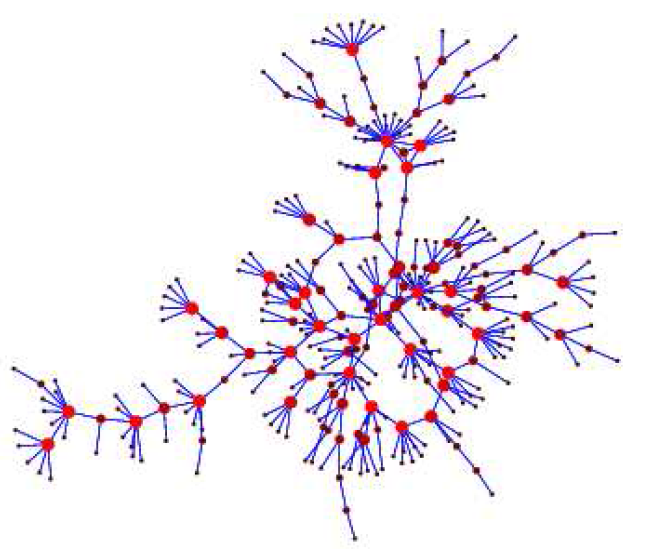
\includegraphics[scale=0.3]{Capitulo2EstadoDelArte/imagenes/contactos.png}
    \caption{Ejemplo de red de contactos sexuales \cite{Newman2003}}
    \label{fig:contactosSexuales}
\end{figure}

\subsubsection{Definición formal}

Una red o grafo se puede definir así:

\begin{equation}
    G = (V,E)
\end{equation}

Donde $V$ es el conjunto de nodos y $E$ es el conjunto de aristas. Una arista es un par de vértices $(i,j)\in V^2$, en el caso de los grafos dirigidos este par es ordenado. Los enlaces también pueden tener un paso asociado, el cual es un valor numérico. Las redes tienen las siguientes propiedades básicas:

\begin{enumerate}
    \item Dos vértices distintos son adyacentes si y sólo si hay una arista que los conecta
    \item Una arista es incidente a un vértice, si este hace parte de ella
    \item El vecindario de un vértice son todos aquellos que se conectan directamente a través de una arista
\end{enumerate}

\subsubsection{Propiedades de redes complejas}

Las propiedades de una red compleja son\cite{barabasi2002linked}:

\begin{itemize}
    \item Distribución de grado: es la probabilidad que un nodo tenga un número determinado de conexiones
    \item Coeficiente de agrupación: es la probabilidad que tomando un número determinado de nodos se obtenga un grafo completo, el cual consiste en que todos lo nodos se conectan entre sí.
    \item Longitud promedio de la red: Es el promedio de todas las distancias minimas entre los vértices
\end{itemize}

\subsubsection{Clasificación de las redes complejas}

Las redes se clasifican de acuerdo a sus propiedades estructurales en

\begin{enumerate}
    \item Redes aleatorias, las cuales tienen una distribución de grado Poisson
    \item Redes libres de escala: las cuales tienen una distribución de grado de ley de potencia.
    \item Redes de mundo pequeño: son aquellas redes cuyo coeficiente de agrupamiento es levado y la distancia promedio entre los vértices es un valor proporcional al logaritmo del número de nodos.
\end{enumerate}

\subsubsection{Modelos de generación de redes complejas}

Actualmente existen muchos modelos en la literatura, los más relevantes son:

\begin{enumerate}
    \item Modelo de Erdos-Renyi\cite{Erdos1959}: es utilizado para generar redes aleatorias. El método consiste en conectar los nodos entre sí con igual probabilidad. La distribución de grado que se genera en estas redes es Poisson.
    \item Modelo de Albert-Barabasi\cite{Barabaacutesi1999}: permite generar redes libres de escala, mediante un mecanismo de enlace preferencial, en el cual los nodos que tienen mayor grado son los que tienen mayor probabilidad de recibir nuevas conexiones, generando así una distribución de grado de ley de potencia.
    \item Modelo Watts y Strogat\cite{Watts1998}: el cual genera redes libres de escala mediante un mecanismo de colocar y quitar enlaces, de tal forma la distancia promedio entre cada par de nodos sea la menor posible.
\end{enumerate}

\newpage

\section{Estado del arte de análisis fractal y multifractal de redes complejas}

\subsection{Análisis multifractal}

Muchos estudios han demostrado que las redes complejas permiten modelar y caracterizar la dinámica de sistemas complejas presentes en la vida real\cite{BarabasiNetwork}. Los nodos de una red representan los elementos o agentes y las aristas representan la relación entre estos. Las aristas tienen un significado dentro del sistema y su existencia se debe a una relación o una regla que rige los agentes. Las redes complejas pueden ser estudiadas a partir de sus propiedades estructurales, como lo son la distribución de grado, las medidas de centralidad, su diámetro, la existencia de comunidades dentro de la red, entre otras. Recientemente, las redes complejas han sido estudiadas desde sus propiedades geométricas, una de estas medidas es la fractalidad o autosimilaridad, la cual permite estudiar cómo es la estructura interna de una red compleja\cite{Estrada2011}.

Para la medida de fractalidad, Song y otros\cite{Song2005} han propuesto un algoritmo generalizado de conteo de cajas. Este algoritmo es ampliamente utilizado en espacios geométricos, los cuales son transformados en espacios de acuerdo a la distancia más corta entre cada par de nodos, para así ser aplicado en redes complejas. Ellos encontraron que muchas redes complejas son auto-similares bajo ciertos valores de escala. En un trabajo posterior de los mismos autores\cite{Song2007}, se proponen una serie de algoritmos para calcular la dimensión fractal, entre los cuales se tiene, una aproximación al problema de coloreo de grafos y un algoritmo de conteo basado en el solapamiento de las cajas.

Posteriormente, Kim y otros\cite{Kim2007A}\cite{Kim2007B} proponen un algoritmo para la dimensión fractal en redes libres de escala basada en su esqueleto, el cual es obtenido a partir del árbol generador mínimo. Esta aproximación permite determinar la dimensión fractal más rápidamente que las anteriores estrategias, debido a que no se requiere explorar toda la red. A partir de esta idea, Zhou y otros\cite{Zhou2007} diseñan un algoritmo basado en el problema de cobertura de aristas, el cual es aplicado en redes complejas biológicas. 

Según Lee y Jung\cite{Lee2006} la dimensión fractal no es suficiente para describir las propiedades de autosimilaridad en redes complejas, se propone como herramienta el análisis multifractal, el cual además de considerar la dimensión fractal toma en cuenta la escalabilidad. Se encuentra preliminarmente que el análisis multifractal permite describir de mejor forma la distribución del coeficiente de agrupamiento en una red compleja.

Para el análisis multifractal se han propuesto algunos algoritmos para calcular los exponentes de masa\cite{Liu2014}, los cuales describen los cambios de densidad de la red compleja a medida que esta es escalada. Basado en los algoritmos de conteo de cajas para análisis fractal, se ha introducido una variante denominada algoritmo de conteo de cajas compacto\cite{Furuya2011}. Esta variante, toma como exponentes de masa el promedio del número de nodos elevado a un factor que representa la escala y calcula la dimensión fractal a partir de una regresión lineal entre el logaritmo de los exponentes de masa y el logaritmo del tamaño de las cajas, sin embargo, debido al gran número de computaciones que se deben realizar, este algoritmo no es práctico para redes grandes.

Buscando reducir el número de computaciones en el análisis multifractal en redes complejas, Liu y otros\cite{Liu2015} proponen una solución para redes complejas basado en el algoritmo propuesto para objetos geométricos de Tel y otros\cite{Tl1989}. Esta solución, la cual denominan como caja de arena, busca reducir el número de computaciones al no tener que calcularse el número mínimo de cajas de un radio determinado que se requiere para cubrir la red, sin embargo, se requiere repetir el proceso varias veces para obtener una buena estimación de las dimensiones.

\subsection{Aplicaciones prácticas}

El análisis multifractal se aplica en diferentes áreas del conocimiento, a continuación algunos trabajos recientes por área:

\begin{itemize}
    \item En biología, el análisis multifractal es aplicado para analizar relaciones en diferentes ámbitos\cite{Barat2016}, como son las relaciones en ecosistemas, entre proteínas\cite{Wang2014}, etc. Un trabajo destacado, es el estudio del genoma humano realizado por Moreno y otros\cite{Moreno2011}, en el cual se caracteriza la estructura de los diferentes cromosomas, encontrando que se puede categorizar de acuerdo a baja, media o alta multifractalidad, la cual se ve traducida en términos de estabilidad genética, es decir resistencia a factores ambientales que puedan modificar el ADN. Con estudios de este tipo se puede caracterizar algunas particularidades genéticas.
    \item En economía, la variación de precios en los mercados se ha estudiado desde diferentes enfoques, pasando por análisis de promedios por ventajas o estadístico, sin embargo, estos métodos presentan problemas debido a que estas son series de tiempo\cite{Siokis2014}. Un enfoque que ha permitido describir el comportamiento de estas, ha sido el análisis multifractal, un ejemplo de ello son el análisis de la red de pagos de Estonia\cite{RendondelaTorre2017}, en este articulo se encuentra que hay un patrón multifractal en esta red de pagos, por lo que toda la economía de este país, presenta un comportamiento multifractal. También, un hallazgo interesante, es que los exponentes de masa tienen un valor muy elevado, lo que indica que la red es bastante irregular. Finalmente, se concluye que este tipo de redes pueden ser estudiadas desde su esqueleto, lo que reduce considerablemente el número de computaciones que se requieren para obtener las dimensiones fractales.
    \item En la comunicación entre especies, se ha encontrado que el habla y los sonidos de algunos animales presenta patrones multifractales, un caso son los sonidos que emiten las aves migratorias\cite{Roeske2018}. El análisis multifractal permite concluir que los sonidos muestran comportamientos globales que varían de acuerdo al tono o la longitud del canto.
    \item El análisis multifractal se utiliza para estudiar la estructura de diferentes redes que modelan el tráfico en redes de telecomunicaciones\cite{DinhDang2004}, sistemas de tráfico\cite{Vojak1994} y redes sociales\cite{Wei2017}. En estas redes reales, se ha encontrado patrones monofractales en redes que son de mundo pequeño y multifractales en las que presentan semejanzas con redes libres de escala.
\end{itemize}


\subsection{Herramientas para el análisis fractal y multifractal}

En la exploración del estado del arte no se evidencia la existencia de una herramienta comercial para usuario final para el análisis multifractal. Lo que se encuentra son implementaciones realizadas por los investigadores de este tema y un complemento para el software Matlab\cite{matlab}. En la tabla \ref{tab:herramientasFractal} se pueden observar algunas de ellas:


\begin{longtable}{|p{3cm}|p{4cm}|p{2cm}|p{2cm}|p{4cm}|}
    \hline
    \textbf{Nombre} & \textbf{Descripción} & \textbf{Tipo de acceso} & \textbf{Lenguaje de programación} & \textbf{Funciones que provee} \\
    \hline
    \endhead
    Multifractal.jl\cite{multifractaljl} & Librería para el análisis multifractal de series de tiempo & Paga\footnote{La librería es gratuita, pero Matlab\cite{matlab} es un software pago \label{foot:matlab}} & Matlab & Determinar el espectro multifractal y dimensiones fractales.  \\
    \hline
    Multifractal Tool\cite{zenodo} & Herramienta para el análisis multifractal de series de tiempo y de imágenes & Paga\footnotemark[1] & Matlab &Provee análisis multifractal utilizando el espectro calculado con la transformada Wavelet, así mismo provee la reconstrucción multifractal de series de tiempo e imágenes. \\
    \hline
    Multifractal estimation using a standard box-counting algorithm\cite{lsaravia} & Esta librería permite realizar un análisis multifractal de un conjunto de imágenes & Libre & R y C++ & Permite calcular los exponentes de masa $T_q$ y dimensiones fractales $D_q$. Es trabajado en el articulo Multifractal analysis of spatial patterns in ecological communities\cite{Saravia2014}. \\
    \hline
    Multifractal Analysis ToolBox\cite{toolbox} & Complemento de Simulink para el análisis multifractal de señales (series e imágenes) & Paga & Matlab & Provee la gráfica de dimensión fractal, el cual denominan espectro multifractal. \\
    \hline
    Multiscale Multifractal Analysis (MMA)\cite{MMA} & Librería de análisis multifractal del Banco de Datos Physionet & Paga\footnotemark[1] & Matlab & Implementación del método propuesto en el articulo Multiscale multifractal analysis of heart rate variability recordings with a large number of occurrences of arrhythmia\cite{Gieratowski2012} \\
    \hline
    MDFA in Python\cite{pythonMFDA} & Modulo de Python para el análisis multifractal de series de tiempo e imágenes & Libre & Python & Esta es la implementación utilizada en al artículo Multifractal analysis for all. Frontiers in Physiology\cite{Jurica2015} \\
    \hline
    Implementation in Python of analysis multifractal\cite{pythonFractal} & Módulo en Python para análisis fractal de redes complejas & Libre & Python & Son las implementacion de los métodos propuestos en How to calculate the fractal dimension of a complex network- the box covering algorithm\cite{Song2007}.\\
    \hline
\caption{Herramientas para el análisis multifractal encontradas en la literatura}
\label{tab:herramientasFractal}
\end{longtable}

Se puede evidenciar en la exploración realizada, que no se encuentra una herramienta para el análisis multifractal en redes complejas.
\section{Análisis de robustez de redes complejas}

\subsection{Medida de la robustez}

El objetivo del análisis de robustez, es el estudio del efecto en las propiedades estructurales ante la pérdida de nodos y aristas\cite{Albert2000}. Este análisis depende de cada sistema que ha sido modelado con redes complejas, una instancia de esto es el efecto de la falla de enrutadores en el Internet.

Una descripción más precisa, este análisis permite observar si la red complejas continua funcionando a pesar de que algunos componentes individuales han fallado o se han degradado. El enfoque consiste en cómo la estructura de la red cambia a medida que esta pierde vértices y aristas. Varios trabajos relevantes tratar en este tema en sistemas que son modelados como redes complejas, como es el caso de la resilencia de Internet ante caídas de enlaces o fallas aleatorias\cite{Cohen2000} y de cómo fortalecer estos sistemas para conservar su funcionamiento en eventos de talla\cite{Cohen2003}.

Mark Newman en su libro Networks: An introduction\cite{Newman2010} realiza una profunda revisión en el capitulo 16, el cual trata sobre la percolación y resilencia en redes complejas. Varias estrategias de estudio son la perdida aleatoria de vértices y la pérdida de acuerdo al grado. Un enfoque de estudio es cómo se muestran las medidas estructurales dentro del componente gigante, el cual es el componente conexo más grande y a partir de allí se establece un análisis de la robustez de una red.

Para formalizar esta medida, inicialmente se tienen en cuenta que desde la década de 1980, se tienen algunas métricas de conectividad. Algunas de ellas son la conectividad algebraica\cite{Fiedler1973}, la superconectividad\cite{Bauer1985}, conectividad condicional\cite{Harary1983} y número isoperimétrico\cite{Mohar1989}. Sin embargo, estas medidas de robustez basadas en la conectividad sólo consideran la estructura topológica de la red y no tienen en cuenta el nodo o enlace que falla. Para atacar este problema, Albert y otros\cite{Albert2000} proponen considerar las propiedades estadísticas como marco de trabajo para el medida de robustez. 

Siguiendo la idea de analizar las propiedades estadísticas de las redes complejas, Schneider y otros\cite{Schneider2011} proponen una métrica de robustez basada en el tamaño del componente gigante, de la siguiente forma:

\begin{equation}
 R = \frac{1}{N} \sum \limits_{i=1}^{N} \delta(\frac{i}{N}) 
\end{equation}
En el cual se tiene un factor de normalización que depende del número de nodos $N$, y $\delta(\frac{i}{N})$ es la medida de una propiedad estructural en el componente gigante a medida que se pierde un número determinado de nodos. Este índice es una aproximación ampliamente utilizada para la medición de la robustez de una red compleja. Sin embargo, ellos no proveen información en un algoritmo detallado para calcular esta métrica. Para resolver este problema, Li y otros\cite{Li2012} desarrollan un algoritmo que permite realizar este proceso.

\subsection{Aplicaciones del análisis de robustez}

Gran parte de las aplicaciones de análisis de robustez nacen a partir del trabajo de Schneider y otros\cite{Schneider2011}, a continuación se mencionan algunos trabajos relevantes por área:

\begin{itemize}
    \item En seguridad, el trabajo de Li y otros\cite{Li2016} abarca el problema del estudio de la entropía de la información a la cual se le aplica un patrón de ruido conocido y como este afecta su estructura la cual se modela a través de una red compleja. De esta forma, ellos proponen un índice de resistencia que da una idea de la medida de robustez de una red de comunicaciones.
    \item Para el suministro de energía, Pahwa y otros\cite{Pahwa2014} estudian el estrés que son sometidas las redes de transmisión de energía a medida que aumenta la demanda y las caídas de enlaces. Ellos realizan un estudio con redes reales encontrando una directa relación entre la caída total del sistema y la medida de robustez de la red.
    \item En salud pública, un tema de gran interés es el estudio de la propagación de epidemias dentro de comunidad. En un estudio realizado por Chami y otros\cite{Chami2017} se estudian las estrategias que pueden aplicar las organizaciones encargadas de velar por la salud pública. Algunas de estas estrategias consisten en aislar a los individuos enfermos o fomentar que estas personas eviten contacto con otros, sin embargo, ellos encuentran a partir de un caso de estudio que consiste en una red de amistades de comunidades rurales en Uganda que un enfoque más eficiente para controlar la propagación de epidemias es vacunar o aislar aleatoriamente a ciertos individuos que tienen contacto con muchas personas así no estén enfermos, como es el caso de profesores, funcionarios de gobierno entre otros. Al aplicar este enfoque en la comunidad de estudio, se encuentra que la efectividad de la propagación de enfermedades se reduce, ya que esto produce un mayor efecto en la red de propagación.
\end{itemize}
\section{Algoritmos de inteligencia artificial en redes complejas}


\subsection{Patrones en redes complejas}

En las redes complejas se pueden identificar patrones estructurales, los cuales pueden ser
utilizados para su estudio. Li y otros\cite{Li2012IA} realizan un evaluación de las redes complejas de gran escala utilizando herramientas de minería de datos y reconocimiento de patrones, a través de una conversión de las redes en estructuras de nubes de datos, que facilita el proceso de descubrimiento de patrones en las redes. Como resultado de este trabajo se encuentra que si se proyectan las redes en un espacio multidimensional de parámetros se pueden encontrar patrones.

Otro aporte relevante en fue la conferencia \textit{Workshop on Structural, Syntactic, and Statistical Pattern Recognition}\cite{Jain2000}, realizada
en el año 2010, donde se presentaron trabajos sobre la descripción estructural de redes complejas y el uso de estrategias de inteligencia artificial para su estudio. Un ejemplo de ello son el uso de redes Markovianas para el estudio de redes complejas enmarcados en el estudio de la categorización de material multimedia en el estándar MPEG-7. Otro campo de estudio de esta conferencia fue el estudio del aprendizaje estructural, con el uso de ténicas como los vectores de cuantización (LVQ) para la descripción estructura del grafos, los resultados indican que se
pueden utilizar para la descripción de grafos.


Desde el enfoque del estudio de sistemas biológicos, Wuchty y otros\cite{Wuchty2005} realizan un estudio de la aplicación de diferentes técnicas a sistemas complejos que representan interacciones entre proteínas. Se busca integrar las redes complejas, el análisis de imágenes, el procesamiento de señales y la inteligencia artificial, mediante el estudio de aplicación de estas técnicas a varios casos de estudio, uno de ellos, consiste en estudiar esencialidad de las proteínas, que consiste en construir una red compleja a partir de sus interacciones. El análisis de este caso indica que existen propiedades como
la centralidad de nodos y propiedades de \textit{k-core} en la red, las cuales permiten describir la topología de la red.

\subsection{Algoritmos de inteligencia artificial aplicados en redes complejas}

Los trabajos donde se han utilizado técnicas de inteligencia artificial para la medición de parámetros en redes complejas están basados principalmente en estrategias para optimizar algoritmos ya existentes, como es el caso del trabajo de Zhou y otros\cite{Zhou2007}, en donde se explica la autosimilaridad en redes complejas celulares mediante un método de cobertura de aristas utilizando algoritmos de recocido simulado aplicado dentro del algoritmo cobertura de cajas. Esta técnica consiste en encontrar un número mínimo de $N$ cajas de tamaño $l$ que pueda cubrir las aristas de la red. Las pruebas se realizaron sobre 43 redes celulares, encontrando que estas redes presentan una distribución de ley de potencia, donde la dimensión fractal es $[2,67 \pm 0,15]$. Sin embargo, este resultado no puede concluir que exista una distribución de grado de ley de potencia en todas las redes celulares.

Para los algoritmos evolutivos, un elemento de la literatura clave es libro \textit{Multiobjective Evolutionary Algorithms on Complex Networks} de  Michell Kirley y Robert Stewart\cite{Michel2007}, en donde se realiza una introducción del uso
de algoritmos evolutivos multiobjetivo en redes complejas. Este libro ofrece diferentes acercamientos teóricos para permitir mapear los nodos de una red dentro de los individuos de una población, crear reglas de selección y evolución de tal manera se pueda modelar una red compleja y así aplicar algoritmos para la medición de parámetros en ellas.

En la aplicación técnicas de inteligencia artificial en problemas de redes complejas es el realizado por Chien\cite{Chien1998}, en el cual se plantea el uso de técnicas de planificación basadas en inteligencia
artificial, en redes donde se representan las interacciones entre diferentes componentes de software. Se utiliza un algoritmo conocido como \textit{Multimission VICAR Planner}(MVP) utilizado en el procesamiento digital de imágenes, este algoritmo permite a partir de un conjunto
de imágenes de interés y la especificación de un estado deseado, realizar un conjunto de pasos para alcanzar dicho estado; en este algoritmo se construye un grafo que representa la estructura de almacenamiento de las imágenes. La aplicación MVP al problema de componentes de software permite estructurarlos considerando sus dependencias
y categorías. Los resultados muestran una mejoría en el proceso de configuración y reconfiguración de estos módulos. Otro trabajo relevante, es el realizado por Jian Liua y Tingzhan Liub\cite{Liu2010}, dónde se utilizan una combinación entre el algoritmo de recocido simulado y el algoritmo K-Means para encontrar comunidades dentro de redes complejas. Las comunidades se pueden ver cómo grupos de nodos que comparten características similares representadas por el peso de las conexiones dentro de la
red. En este trabajo, se encuentra que el uso de estas técnicas combinadas ayudan a encontrar más rápidamente las comunidades dentro de la red debido a que mejora la elección del centro de cada clúster en el procesos del algoritmo K-Means, debido al proceso de calentamiento o enfriamiento que provee el algoritmo de recocido simulado, y además, se pueden encontrar comunidades sin las necesidad de conocimiento previo acerca de la estructura de las comunidades.

En el diseño heurísticas para aplicar algoritmos de inteligencia artificial en redes complejas, en la literatura se encuentran varios trabajos relevantes, uno de ellos es realizado por Chen y otros\cite{Chen2009}, el cual se propone una heurística para la detección de comunidades en redes complejas utilizando como base la existencia de relaciones cercanas entre los nodos de una misma comunidad, para calcular el centro de cada comunidad en base las relaciones entre nodos y no directamente al promedio de los parámetros de cada nodo. Los resultados de esté articulo demuestran a-priori que el uso de esta estrategia sobre cuatro redes de prueba, es más eficiente para la detección de comunidades en redes complejas que otras estrategias como es el caso del algoritmo K-Means, debido a que los centros de cada comunidad convergen más rápidamente.

\newpage
\section{Resumen y conclusiones del capitulo}

En este capitulo se ha dado un marco referencial para entender el concepto de red compleja y así poder abordar el análisis de multifractalidad y robustez. También, se ha mostrado cómo se encuentra el estado del arte en estos temas. A continuación, algunos comentarios:

\begin{itemize}
    \item El análisis de redes complejas se realiza con las herramientas que provee la teoría de grafos. Sus propiedades estructurales y la clasificación está basada con las que comúnmente se trabajan con grafos.
    \item En el estado del arte, el análisis fractal y multifractal es basado en métodos geométricos de cobertura de cajas, en los cuales se realiza un mapeo espacial de un sistema euclidiano a uno basado en la distancia más corta entre cada par de nodos.
    \item Así mismo, el análisis de robustez es el estudio de cómo cambian las propiedades estructurales de la red a medida que esta pierde nodos o conexiones, el significado de estos valores depende directamente de lo que se está modelando con la red.
    \item Finalmente, en la literatura se encuentra que la relación entre la medida de fractalidad y robustez no ha sido ampliamente explorada, por lo que realizar un estudio en esta materia permite generar un aporte teórico para la generación de nuevas métricas y algoritmos.
    \item Así mismo, en la literatura no se evidencia la existencia de una herramienta que realice un análisis de multifractalidad y robustez en redes complejas.
\end{itemize}

%%%%%%%Capitulo TRES: Generación redes fractales%%%%%%
\chapter[Generación de redes fractales]{Generación de redes fractales}
\label{cap3}
\markboth{Generación de redes fractales}{Generación de redes fractales}
\section{Redes fractales}

Los fractales en naturaleza son estructuras que mantienen su forma a diferentes escalas. En el caso de las redes, existe una familia conocida como $(x,y)-$flowers\cite{Rozenfeld2007}, la cuales son conocidas como redes libres de escala jerárquicas. Rozenfeld y otros\cite{Rozenfeld2007B} han demostrado analíticamente que estas redes conservan sus propiedades analizando el escalado de los hubs y los nodos.

Un método de construcción iterativo de estas redes es propuesto por Lin y otros\cite{Lin2011} en un estudio de árboles de cobertura mínima en redes complejas autosimilares.

Este método, consiste en generar una función $F(x,y)$ donde $x>0$ y $y>0$ que permite construir la flor dadas $n$ generaciones. Para $n=0$ la red que genera $F_0(x,y)$ siempre tiene dos vértices unidos por una arista.  A medida que se itera $F_n(x,y)$ se deriva al reemplazar cada arista existente en $F_{n-1}$ por caminos de largo $x$ e $y$. El número de aristas del algoritmo generador siempre es $|E| = (x+y)^n$. 

\begin{figure}[H]
    \centering
    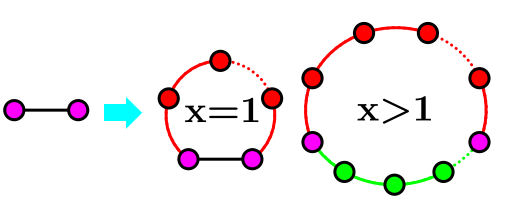
\includegraphics[scale=0.5]{Capitulo3GeneracionRedesFractales/imagenes/florA.png}
    \caption{Proceso iterativo de construcción de las $(x-y)$-flowers. Tomado de \cite{Lin2011}}
    \label{fig:floarA}
\end{figure}

En la figura \ref{fig:floarA} el proceso iterativo consiste en reemplazar cada arista con un camino de tamaño $x, x\leq 1$ y $y, y\leq x \wedge y > 1$. Para $x=1$ un par de nodos de la iteración anterior es directamente conectado con $y-1$ nuevos nodos. Todos estos nuevos nodos y dos de los nodos de la iteración anterior forma un camino rojo de tamaño $y$. Para $x>1$ cada arista antigua es reemplazada por dos caminos que consisten en $y-1$ nodos.

Otra forma de construir las redes es ir formando la red con copias de ella misma. En la figura \ref{fig:florGeneradas} se observa este proceso.

\begin{figure}[H]
    \centering
    \begin{subfigure}[b]{0.5\textwidth}
        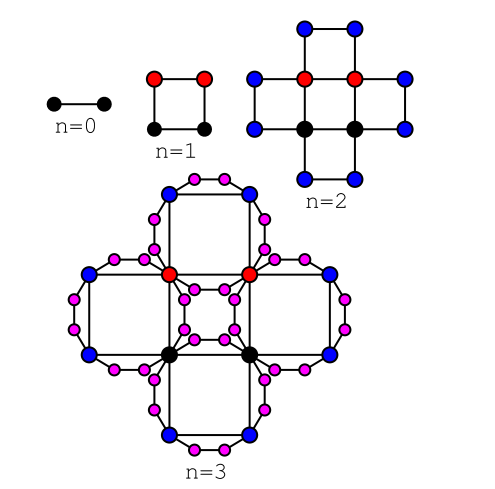
\includegraphics[width=\textwidth]{Capitulo3GeneracionRedesFractales/imagenes/florB.png}
        \caption{Generación de $(1,3)-$flower}
    \end{subfigure}~
    \begin{subfigure}[b]{0.5\textwidth}
        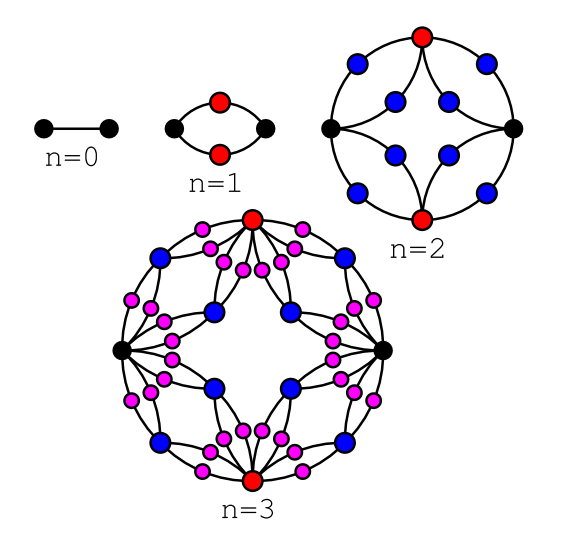
\includegraphics[width=\textwidth]{Capitulo3GeneracionRedesFractales/imagenes/florC.png}
        \caption{Generación de $(2,2)-$flower} 
    \end{subfigure}
    \caption{Proceso iterativo de generación de redes $(x,y)$-flowers. Tomado de \cite{Lin2011}}
    \label{fig:florGeneradas}
\end{figure}
\section{Algoritmo para generar redes fractales}

Para la generación de redes fractales se utiliza la matriz de adyacencia para realizar este proceso. La matriz de adyacencia $M$ de un grafo o red $G(V,E)$ no dirigido es de tamaño $|V|\times|V|$. Para cada $(i,j)\in V^2$ se tiene que $M_{i,j}=1$ si existe una arista entre $i$ y $j$, en caso contrario $M_{i,j}=0$. 
Dado que la matriz de adyacencia para grafos no dirigidos tiene simetría triangular superior, sólo se requiere recorrer las filas $i$ y columnas $j$ que cumplan $i<j$.

\subsection{Red (2,2)-flower}

Para la generación 0, se toma como caso base la siguiente matriz de adyacencia:

\begin{figure}[H]
    \centering
\[ 
\left( \begin{array}{cc}
 0 & 1  \\ 
 1 & 0 \\
\end{array} \right)\]
\caption{Matriz de adyacencia para la generación 0 de (2,2)-flower}
\end{figure}

Para cada generación, se recorre la matriz de tal forma que cuando se encuentra un $1$ en una posición $(i,j)$ cualesquiera, esta es cambiada por 0, es decir que se elimina la arista, es de anotar, que también se hace lo mismo con $(j,i)$ dado que simétrica.  Después se agregan dos filas llenas de ceros $k$ y $k+1$. Dado que la matriz es simétrica agregar una fila implica agregar una columna. En las siguientes posiciones se coloca 1:

\begin{itemize}
    \item En las posiciones $(i,k)$, $(k,i)$, $(i,k+1)$, $(k+1,i)$, $(j,k)$, $(j,k+1)$, $(j,k+1)$ y $(j,k+1)$,
\end{itemize}

\begin{figure}[H]
    \centering
     \begin{subfigure}[b]{0.25\textwidth}
\[ 
\left( \begin{array}{cc}
 0& \textbf{1}  \\ 
\textbf{1} &  0 \\
\end{array} \right)\]
\caption{Generación 0}
 \end{subfigure}~ \begin{subfigure}[b]{0.25\textwidth}
 \[ \left( \begin{array}{cccc}
 0 &  \textbf{0} & 1 & 1  \\ 
\textbf{0} & 0 & 1 & 1\\
 1 & 1 & 0 & 0 \\
 1 & 1 & 0 & 0\\
\end{array} \right)\]
\caption{Generación 1}
     \end{subfigure}
    \caption{Proceso para construir la generación 1 de (2,2)-flower. Observe que las aristas eliminadas son resaltadas en negrilla}
    \label{fig:redesfractalesA}
\end{figure}

En la figura \ref{fig:redesfractalesA} se muestra  que cada arista en la generación anterior es eliminada.

En la tabla  \ref{tab:flower22} se puede observar algunas propiedades estructurales de las primeras 4 generaciones de (2,2)-flower.
\begin{table}[H]
    \centering
    \begin{tabular}{|p{2cm}|p{2cm}|p{2cm}|p{2cm}|p{2cm}|p{3cm}|}
    \hline
        \textbf{Generación} & \textbf{Número de vértices} & \textbf{Número de aristas} & \textbf{Grado promedio} & \textbf{Diámetro de la red} & \textbf{Longitud media de caminos}\\
        \hline
        0 &2 & 1 & 1 & 1 & 1\\
        \hline
        1 &4 & 4 & 2 & 2 & 1.33\\
        \hline
        2 &12 &16 &2.67 & 4 & 2.3\\
        \hline
        3 &44 &64 & 2.91 & 8& 4.35 \\
        \hline
    \end{tabular}
    \caption{Propiedades estructurales de generaciones 0,1,2 y 3 de la red fractal (2,2)-flower}
    \label{tab:flower22}
\end{table}


\subsection{Red (1,3)-flower}

Para la generación 0, se toma como caso base la siguiente matriz de adyacencia:

\begin{figure}[H]
    \centering
\[ 
\left( \begin{array}{cc}
 0 & 1  \\ 
 1 & 0 \\
\end{array} \right)\]
\caption{Matriz de adyacencia para la generación 0 de (1,3)-flower}
\end{figure}

Para cada generación, se recorre la matriz de tal forma cuando se encuentra un $1$ en una posición $(i,j)$ cualesquiera se deben crear dos vértices, los cuales se conectan centre sí, uno de los vértices se conecta con el vértice $i$ y el otro con el vértice $j$. 

Como se deben agregar dos vértices, se crean filas llenas de ceros $k$ y $k+1$. Dado que la matriz es cuadrada agregar una fila implica agregar una columna. Para crear el camino de longitud 1, en las siguientes posiciones se coloca 1:

\begin{itemize}
    \item Para generar un camino de longitud 2, para las posiciones $(k,k+1)$ y $(k+1,k)$ 
    \item En las posiciones $(i,k)$, $(k,i)$, $(j,k+1)$ y $(j,k+1)$, para conectar los nodos antiguos con un camino de longitud 2 $(y-1)$.
\end{itemize}

\begin{figure}[H]
    \centering
     \begin{subfigure}[b]{0.25\textwidth}
\[ 
\left( \begin{array}{cc}
 0 & \textbf{1}  \\ 
\textbf{1} & 0 \\
\end{array} \right)\]
\caption{Generación 0}
 \end{subfigure}~ \begin{subfigure}[b]{0.25\textwidth}
 \[ \left( \begin{array}{cccc}
 0 & \textbf{1} & 1 & 0  \\ 
 \textbf{1} & 0 & 0 & 1\\
 1 & 0 & 0 & 1 \\
 0 & 1 & 1 & 0\\
\end{array} \right)\]
\caption{Generación 1}
     \end{subfigure}
    \caption{Proceso para construir la generación 1 de (1,3), flower. Observe que las aristas que se conservan son resaltadas en negrilla}
    \label{fig:redesfractales}
\end{figure}

El proceso mostrado en la figura  \ref{fig:redesfractales} para las (1,3)-flowers, para cada arista se generan dos vértices conectados por una arista. Las dos aristas se conectan por sus extremos. A continuación se describen las propiedades estructurales de las primeras 4 generaciones de la (1,3)-flower

\begin{table}[H]
    \centering
    \begin{tabular}{|p{2cm}|p{2cm}|p{2cm}|p{2cm}|p{2cm}|p{3cm}|}
    \hline
        \textbf{Generación} & \textbf{Número de vértices} & \textbf{Número de aristas} & \textbf{Grado promedio} & \textbf{Diámetro de la red} & \textbf{Longitud media de caminos}\\
        \hline
        0 &2 & 1 & 1 & 1 & 1\\
        \hline
        1 &4 & 4 & 1 & 2 & 1.2\\
        \hline
        2 &12 &16 &2.67 & 4 & 2.3\\
        \hline
        3 &44 &64 & 2.91 & 6 & 3.11 \\
        \hline
    \end{tabular}
    \caption{Propiedades estructurales de generaciones  0,1,2 y 3 de la red fractal (1,3)-flower}
    \label{tab:flower13}
\end{table}

\newpage

\section{Resumen y conclusiones del capítulo}

%%%%%%%Capitulo Cuatro: Medición de multifractalidad%%%%%%

\chapter{Análisis multifractal}\label{cap4}
\markboth{Análisis multifractal}{Análisis multifractal}

\section{Introducción}

Desde el trabajo pionero de Song\cite{Song2005} se ha considerado que las redes complejas consisten en patrones auto-similares bajo transformaciones de escala. Se han proporcionado diferentes estrategias basadas en la cobertura de cajas para caracterizar la dimensión fractal en redes complejas. Sin embargo, la dimensión fractal no es suficiente para caracterizar las propiedades fractales de las redes complejas, por esta razón para el análisis multifractal se propone calcular la dimensión fractal a medida que se realiza un escalado de la red.

El análisis multifractal es útil para caracterizar la heterogeneidad espacial de las redes complejas, ya que considera que no sólo existe un patrón de estructuras dentro de las redes complejas.

Las diferentes estrategias permiten calcular los exponentes de masa $\tau_q$, que representan como cambia la densidad de la red a medida que se escala por un factor real $q$ y la pendiente de esta recta para un $q$ dado viene siendo la dimensión fractal $D_q$, de esta forma se puede estudiar los cambios en la estructura de la red a medida que esta es escalada.

Si la función $D_q$ es una linea recta, se dice que la red es monofractal, en caso contrario, es multifractal.

\section{Estrategias de cubrimiento de cajas}

Este método es una herramienta para estimar la dimensión fractal de objetos en un espacio Euclidiano. Sin embargo, la métrica no es relevante para redes complejas, por es razón se considera la longitud del camino más corto entre un par de nodos como métrica. 

Para una red cualquiera, se toma $N_B$ como el número de cajas de radio $r_B$ que se necesitan para cubrir toda la red, por lo tanto la dimensión fractal $d_B$ se caracteriza de la siguiente forma:

\begin{equation}
    N_B \approx r_B^{d_B}
\end{equation}

El algoritmo más común para obtener esta medida es:

\begin{enumerate}
    \item Seleccione un nodo aleatoriamente como el centro de una caja
    \item Busque los nodos a un radio $r_B$ y que no han sido cubiertos por otra caja y asígnelos a la caja
    \item Repita los pasos 1 y 2 hasta asignar los nodos a sus respectivas cajas
\end{enumerate}

La dimensión fractal con la pendiente de la regresión lineal entre $log(N_B))$ y $log(d_B)$

De este algoritmo se tienen varias variante que dependen como se seleccionan los centros:

\begin{enumerate}
    \item Selección aleatoria\cite{Kim2007B}: Seleccionando los centro de tal forma se obtenga el mínimo número de cajas.
    \item Estrategia voraz\cite{Song2007}: Seleccionando los centro de acuerdo a un problema análogo de coloreo de grados
    \item Estrategia quemada\cite{Song2007}: Consiste en permitir solapamientos entre las cajas  y cubrir la red con estas.
\end{enumerate}

Los autores de estas estrategias mediante pruebas en algunas redes, han encontrado que se obtiene una medida de dimensión fractal similar a la calculada analíticamente.



\subsubsection{Box Covering Fixed Size}

Uno de los algoritmos que se se ha propuesto, es el de \textit{Box Covering Fixed Size}\cite{Halsey1986}\cite{RendondelaTorre2017}\cite{Yu2003}, el cual consiste en considerar para una medida dada, se considera la siguiente relación:

\begin{equation}
    Z_e(q) =  \sum \limits_{\mu(B) \neq 0} \mu(B)^q
\end{equation}

Donde $q\in R$ y la suma representa todas las diferentes cajas $B$ no vacías, para un tamaño $e$ definido y que cubren toda la red. Los exponentes de masa $\tau(q)$ están definidos por:

\begin{equation}
    \tau(q) = \lim_{x \to \infty} \frac{\ln Z_e(q)}{\ln e}
\end{equation}

Las dimensiones fractales generalizadas están definidas por:

\begin{equation}
    D_q = \frac{\tau(q)}{q-1}, q \neq 1
\end{equation}

Y

\begin{equation}
    D_1 = \lim_{x \to 0} \frac{Z_{1,e}}{ln e}
\end{equation}

Donde $Z_{1,e} = \sum \limits_{\mu(B) \neq 0} \mu(B) \ln \mu(B)$

Los exponentes de masa se pueden obtener a través de una regresión lineal entre $ln(Z_e(q)$ y $ln e$, así mismo las dimensiones fractales 

Debido a que la elección de los centros de las cajas es aleatorio, esto puede afectar la medida. Si se seleccionados vértices con un gran grado (hub) se puede cubrir la red de forma eficiente, pero si son seleccionados nodos con grado bajo, pocos nodos pueden ser cubiertos. Para enfrentar este problema se propone seleccionar un conjunto T de permutaciones distintas de nodos y tomar un promedio. La sección de T, debe estar acorde al número de nodos.

El procedimiento para calcular las dimensiones fractales es:

\begin{enumerate}
    \item Se generan matrices de adyacencia y distancias
    \item En primer lugar, asegurarse que todos los nodos en la red no esté cubiertos por alguna caja
     \item Se generan T permutaciones de vértices (con todos los existentes en la red), los cuales serán seleccionado como centros de cajas en el orden de aparición
     \item Se selecciona el tamaño de una caja $r\in[1,d]$  donde $d$ es el diámetro de la red.
     \item Se selecciona el centro de la caja y se incluyen todos los nodos que están dentro de una distancia $r$ y no han sido cubiertos
     \item Se repite este proceso hasta que todos los vértices han sido cubiertos
     \item Se toma como medida $\mu(B)=\frac{N_B}{N}$ donde $N_B$ es el número de vértices en la red y $N$ es el número total de vértices.
     \item Se calcula la suma $ Z_r(q) =  \sum \limits_{\mu(B) \neq 0} \mu(B)^q$
     \item Se repiten los pasos 3-8 con cada uno de los conjuntos $T$. Se toman los promedios de $\overline{Z_r(q)} = \sum^t (Z_r(q))/T$  
\end{enumerate}

Posteriormente se realiza una regresión lineal entre $\ln \overline{Z_r(q)}$ y $\ln\frac{r}{d}$. Se debe considera el caso especial cuando $q=1$.

El algoritmo es implementado en lenguaje Python y es aplicado en las siguientes redes del Anexo A en la página \pageref{AnexoA}

\subsubsection{Box Covering Compact}

Esta estrategia
\section{Algoritmo SandBox}
\label{cap4:seccionSB}

Liu y otros\cite{Liu2015} han realizado un estudio de los diferentes algoritmos de Boxcounting encontrando que estos requieren un gran tiempo de cómputo, ya que se realiza la búsqueda de una configuración óptima de centros para obtener una estructura de cubrimiento, en la cual cada caja tiene el mismo número de nodos o se obtiene el número mínimo de cajas necesario para el cubrimiento de la red.

Su propuesta conocida como algoritmo de caja de arena o SandBox, consiste en escoger un número de centros de cajas aleatorios y permitir que las cajas se solapen. Dado que se permite solapamientos, como medida se utilizará el promedio del número de nodos en cada caja y con este valor se realiza le medición.

El proceso de este algoritmo es el siguiente:

\fbox{\begin{minipage}{16.5cm}
 \begin{itemize}
     \item Inicialmente, seleccione un porcentaje nodos como centros de las cajas.
     \item Seleccione el radio $r \in [1,d]$ de cada caja de arena que será usado para cubrir la red.
     \item Cuente el número de nodos en cada caja de arena de radio $r$, denote este número como $M(r)$.
     \item Para todos los centros elegidos calcule el promedio estadístico de $\overline{M(r)^(q-1)}$
 \end{itemize}
 \end{minipage}}

 La regresión lineal se realiza entre $\ln(\overline{M(r)^(q-1)})$ y $\ln(\frac{r}{d})$
 
Debido a que éste método elige centros aleatorios, se recomienda repetirlo varias veces para mejorar la precisión.
 

 
\section{Análisis de los algortitmos}\label{sec:cap4analisis}

Para analizar los 3 algoritmos estudiado Box Counting Fixed Size (BCFS), Box Covering Compact (BCC) y SandBox(SB); se seleccionan algunas redes de prueba, las cuales pueden ser consultadas en el Anexo A de la página \pageref{AnexoA},

La configuración y protocolo de pruebas es explicado en el Anexo B de la página \pageref{AnexoB}

Para este capitulo se han seleccionado las siguientes pruebas:

\begin{enumerate}
    \item Red A: Red libre de escala generada 4000 nodos.
    \item Red B: Red de mundo pequeño generada con probabilidad de reconexión de 10\%.
    \item Red C: Red aleatoria generada con 5620
    \item Red D: Red observada en la bacteria Ecoli.
    \item Red E: Red fractal generada (2,2)-flower.
\end{enumerate}

\subsection{Redes libres de escala}

Inicialmente, para cada estrategia se analiza la relación entre $q$ y $\ln(Zr(q))$

\begin{figure}[H]
    \centering
    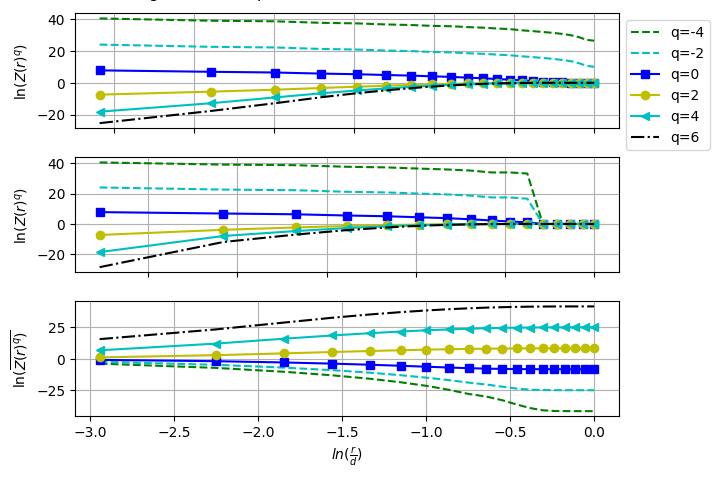
\includegraphics[scale=0.8]{Capitulo4Multifractalidad/imagenes/scaleFree4000_TqLnrBCscaleFree4000Nodes.png}

    \caption{Regresión lineal entre $\ln(Z_r(q)$ y $\ln(\frac{r}{b})$. De arriba hacia abajo, la primera figura corresponde al método BCFS, la segunda al método BCC y la tercera SB}
\end{figure}

Cada valor de $q$ tiene su función de la cual se obtiene su pendiente, la cual corresponde a sus exponentes de masa.

\begin{figure}[H]
    \centering
    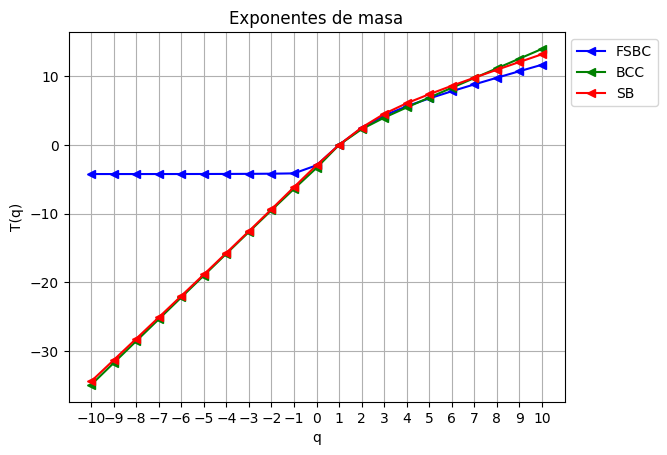
\includegraphics[scale=0.7]{Capitulo4Multifractalidad/imagenes/scaleFree4000_TqscaleFree4000Nodes.png}
    \caption{Exponentes de masa para red libre de escala 4000 nodos}
\end{figure}

Se observa que para el método BCFS los $q<0$ no tienen significado, esto se debe a que en cada caja se toma la cantidad de nodos sobre el total, lo que da valores menores que 1, al elevarlos a un valor $q$ se transforman en valores muy pequeños. Por esta razón, la dimensión se analiza para $q\geq0$

\begin{figure}[H]
    \centering
    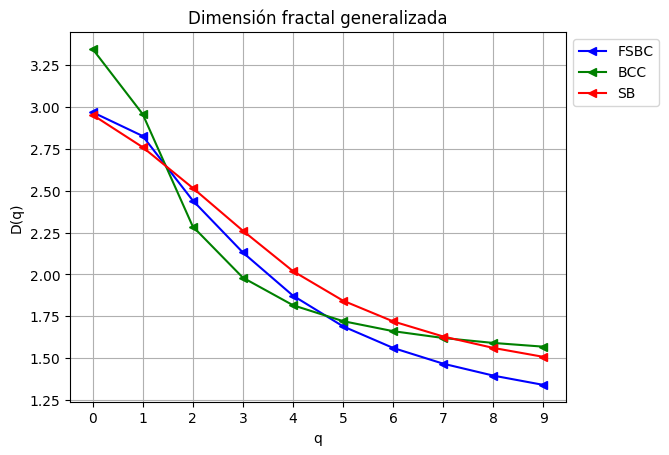
\includegraphics[scale=0.7]{Capitulo4Multifractalidad/imagenes/scaleFree4000_DqscaleFree4000Nodes.png}
    \caption{Dimensión fractal generalizada para red libre de escala 4000 nodos}
\end{figure}

De esta se puede obtener la siguiente información y compararla con el articulo de Wang\cite{Wang2012}:

\begin{table}[H]
    \centering
    \begin{tabular}{|c|c|c|c|c|}
        \hline
         \textbf{Dato}& \textbf{BCFS} & \textbf{BCC} & \textbf{SB} & \textbf{Articulo} \\
         \hline
         Dimensión fractal & 2.97 & 3.34 & 2.95 & 3.19 \\
         \hline
         Dimensión fractal generalizada & 2.82 & 2.95 & 2.75 &3.15  \\
         \hline
         Dimensión de correlación & 2.44 & 2.28 & 2.51 &2.81 \\
         \hline
         Dimensión máxima & 2.97 & 3.34 & 3.14 &3.26 \\
         \hline
         Dimensión mínima & 1.29 & 1.55 & 1.46 &1.75 \\
         \hline
         Variación en la dimensión & 1.68 & 1.79 & 1.68 &1.51 \\
         \hline
    \end{tabular}
    \caption{Comparación de los datos obtenidos con los del artículo de Wang\cite{Wang2012}}
\end{table}

Las diferencias en la medida de la dimensión fractal se deben a que el método es una aproximación y debe ejecutarse muchas veces, además que las redes del articulo y la generada son distintas.

Para evitar estas diferencias Li\cite{Li2014} recomienda que para el caso de $q=0$ se tome directamente la dimensión fractal obtenida por algoritmo de Box Counting, que en este caso es 3.13.

En las gráficas se puede observar que las redes libres de escala son multifractales, algo que es esperado ya que internamente estas redes tienen estructuras diferentes debido a la presencia de hubs altamente conectados.

\subsection{Redes de mundo pequeño}

\begin{figure}[H]
    \centering
    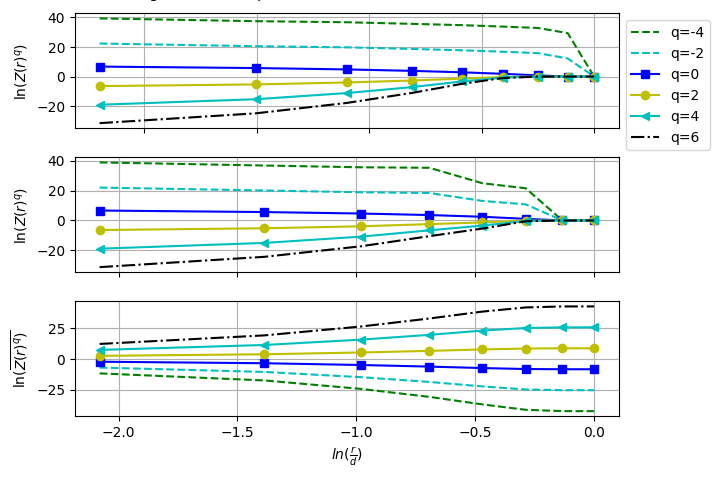
\includegraphics[scale=0.7]{Capitulo4Multifractalidad/imagenes/a_TqLnrBCsmallWorld4000p10.png}
    \caption{Regresión lineal entre $\ln(Z_r(q)$ y $\ln(\frac{r}{b})$. De arriba hacia abajo, la primera figura corresponde al método BCFS, la segunda al método BCC y la tercera SB}
\end{figure}

A continuación, los exponentes de masa:

\begin{figure}[H]
    \centering
    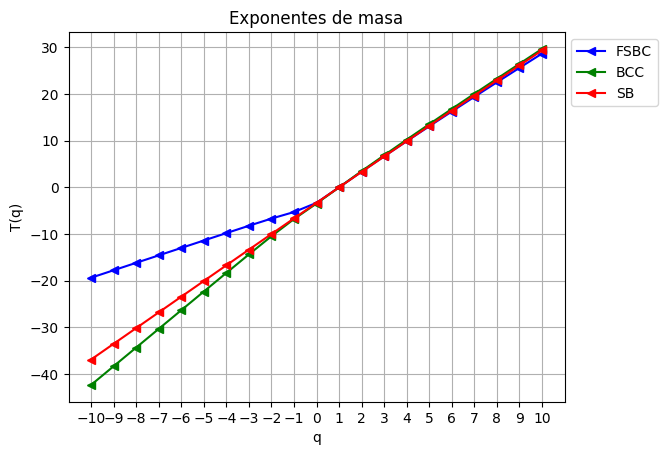
\includegraphics[scale=0.7]{Capitulo4Multifractalidad/imagenes/a_TqsmallWorld4000p10.png}
    \caption{Exponentes de masa para red de mundo pequeño con 5000 nodos y $p=10\%$}
\end{figure}

Finalmente, la dimensión fractal generalizada
\begin{figure}[H]
    \centering
    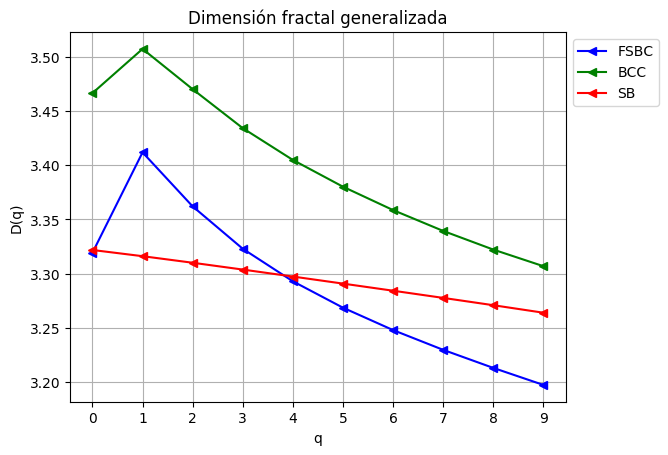
\includegraphics[scale=0.7]{Capitulo4Multifractalidad/imagenes/a_DqsmallWorld4000p10.png}
    \caption{Dimensión fractal generalizada para red de mundo pequeño con 5000 nodos y $p=10\%$}
\end{figure}

De acuerdo a los datos del articulo se encuentra:
\begin{table}[H]
    \centering
    \begin{tabular}{|c|c|c|c|c|}
        \hline
         \textbf{Dato}& \textbf{BCFS} & \textbf{BCC} & \textbf{SB} & \textbf{Articulo} \\
         \hline
         Dimensión fractal &3.31 & 3.46 & 3.32 & 2.79 \\
         \hline
         Dimensión fractal generalizada & 3.41 & 3.5 & 3.31 &2.8  \\
         \hline
         Dimensión de correlación & 3.36 & 3.47 & 3.31 &2.81 \\
         \hline
         Dimensión máxima & 3.41 & 3.84 & 3.35 &2.81 \\
         \hline
         Dimensión mínima & 3.18 & 3.29 & 3.25 &2.75 \\
         \hline
         Variación en la dimensión & 0.23 & 0.55 & 0.1 &0.06 \\
         \hline
    \end{tabular}
    \caption{Comparación de los datos obtenidos con los del artículo de Wang\cite{Wang2012}}
\end{table}

Los resultados varían ya que las redes del articulo y las utilizadas en estas pruebas son generadas, es decir que no son las mismas.

Se observa que la variación en la dimensión fractal es pequeña, de hecho menor que 1, por lo que, se puede concluir que las redes de mundo pequeño son monofractales, es decir que se pueden considerar como una sola estructura. Es importante indicar que las mediciones de los diferentes algoritmos requieren un mayor número de iteraciones para mejorar su presición.

La dimensión fractal de esta red es 3.47

\subsection{Redes aleatorias}

\begin{figure}[H]
    \centering
    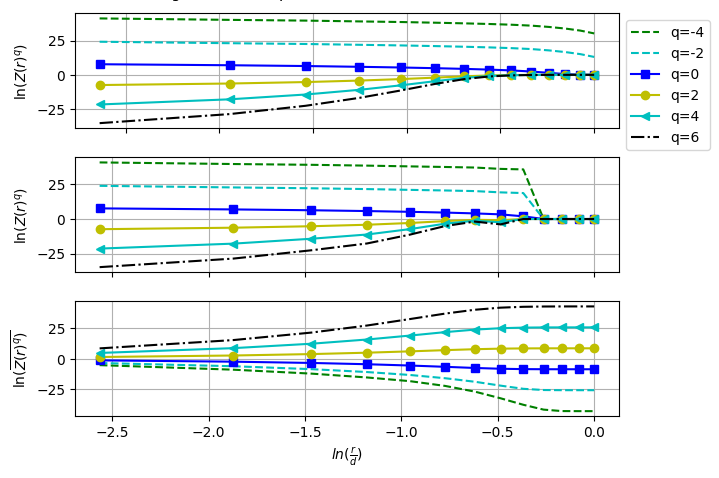
\includegraphics[scale=0.7]{Capitulo4Multifractalidad/imagenes/a_TqLnrBCrandom5620.png}
    \caption{Regresión lineal entre $\ln(Z_r(q)$ y $\ln(\frac{r}{b})$. De arriba hacia abajo, la primera figura corresponde al método BCFS, la segunda al método BCC y la tercera SB}
\end{figure}

\begin{figure}[H]
    \centering
    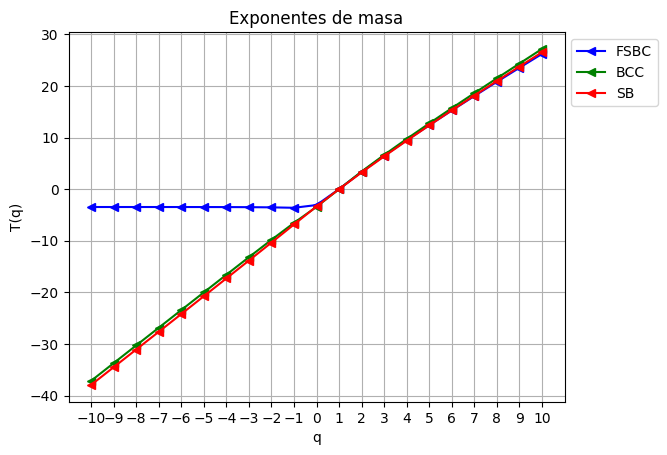
\includegraphics[scale=0.7]{Capitulo4Multifractalidad/imagenes/a_Tqrandom5620.png}
    \caption{Exponentes de masa para red aleatoria de 5620 nodos}
\end{figure}

\begin{figure}[H]
    \centering
    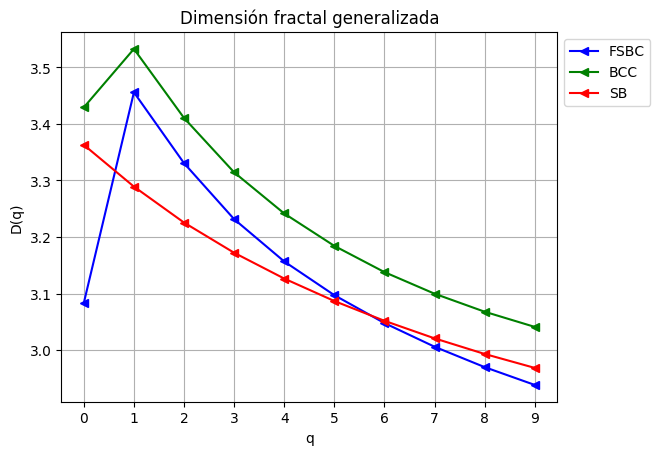
\includegraphics[scale=0.7]{Capitulo4Multifractalidad/imagenes/a_Dqrandom5620.png}
    \caption{Dimensión fractal generalizada para para red aleatoria de 5620 nodos}
\end{figure}

La dimensión fractal de esta red es: 3.41

Los análisis realizados a las redes de prueba, permite concluir que el análisis multifractal no permite caracterizar redes aleatorias, ya que pueden presentar comportamiento monofractal o multifractal. En este caso la red puede considerarse monofractal.

\begin{table}[H]
    \centering
    \begin{tabular}{|c|c|c|c|c|}
        \hline
         \textbf{Dato}& \textbf{BCFS} & \textbf{BCC} & \textbf{SB} & \textbf{Articulo} \\
         \hline
         Dimensión fractal & 3.08 & 3.42 & 3.36 & 3.54\\
         \hline
         Dimensión fractal generalizada  & 3.46 & 3.53 & 3.28 & 3.56 \\
         \hline
         Dimensión de correlación & 3.33 & 3.41  & 3.22 &3.52 \\
         \hline
         Dimensión máxima & 3.45 & 3.53 & 3.46 & 3.54\\
         \hline
         Dimensión mínima & 3.08 & 3.01 & 2.94 & 3.61\\
         \hline
         Variación en la dimensión & 0.37 &  0.52 & 0.52 & 0.33 \\
         \hline
    \end{tabular}
    \caption{Comparación de los datos obtenidos con los del artículo de Wang\cite{Wang2012}}
\end{table}

\subsection{Red observada de Ecoli}

\begin{figure}[H]
    \centering
    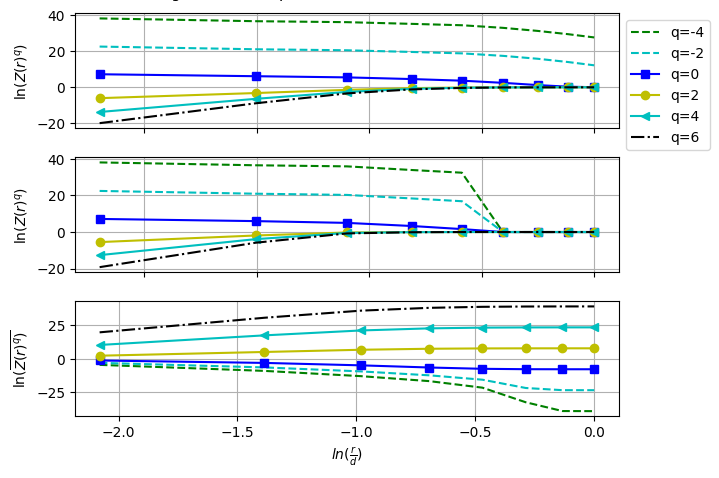
\includegraphics[scale=0.7]{Capitulo4Multifractalidad/imagenes/a_TqLnrBCecoli.png}
    \caption{Regresión lineal entre $\ln(Z_r(q)$ y $\ln(\frac{r}{b})$. De arriba hacia abajo, la primera figura corresponde al método BCFS, la segunda al método BCC y la tercera SB}
\end{figure}

\begin{figure}[H]
    \centering
    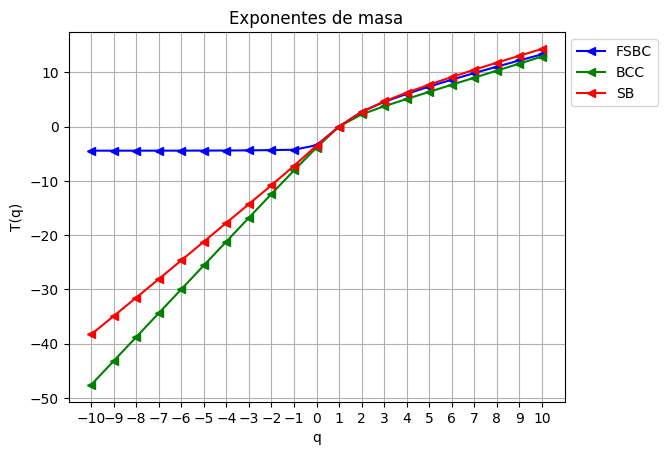
\includegraphics[scale=0.7]{Capitulo4Multifractalidad/imagenes/a_Tqecoli.png}
    \caption{Exponentes de masa para red real ecoli}
\end{figure}

\begin{figure}[H]
    \centering
    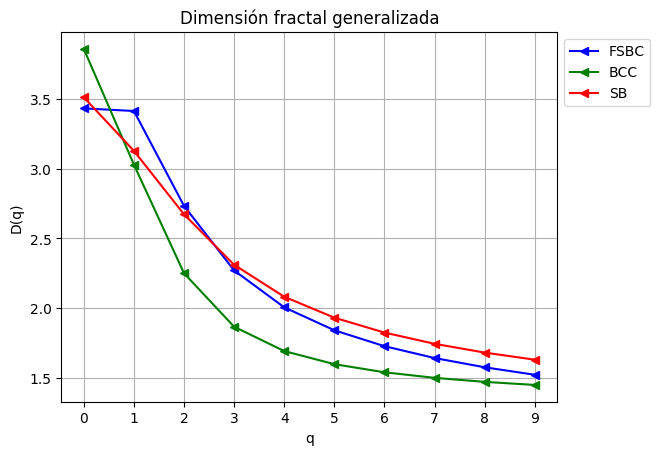
\includegraphics[scale=0.7]{Capitulo4Multifractalidad/imagenes/a_Dqecoli.png}
    \caption{Dimensión fractal generalizada para para red real ecoli}
\end{figure}

La dimensión fractal de esta red es 3.31

\begin{table}[H]
    \centering
    \begin{tabular}{|c|c|c|c|c|}
        \hline
         \textbf{Dato}& \textbf{BCFS} & \textbf{BCC} & \textbf{SB} & \textbf{Articulo} \\
         \hline
         Dimensión fractal & 3.43 & 3.35 & 3.51 & 3.56 \\
         \hline
         Dimensión fractal generalizada  & 3.41 & 3.03 & 3.12 & 3.45 \\
         \hline
         Dimensión de correlación & 2.73 & 2.25 & 2.67 & 2.9 \\
         \hline
         Dimensión máxima & 3.41 & 4.32 & 3.6 & 4.15 \\
         \hline
         Dimensión mínima & 1.47 & 1.43 & 1.5 & 2.1 \\
         \hline
         Variación en la dimensión & 1.94 & 2.91   & 2.1 & 2.05 \\
         \hline
    \end{tabular}
    \caption{Comparación de los datos obtenidos con los del artículo de Wang\cite{Wang2012}}
\end{table}


\subsection{Redes fractales}

Utilizando el articulo de Liu y otros\cite{Liu2015} se trabaja con la (2,2)-flower.

\begin{figure}[H]
    \centering
    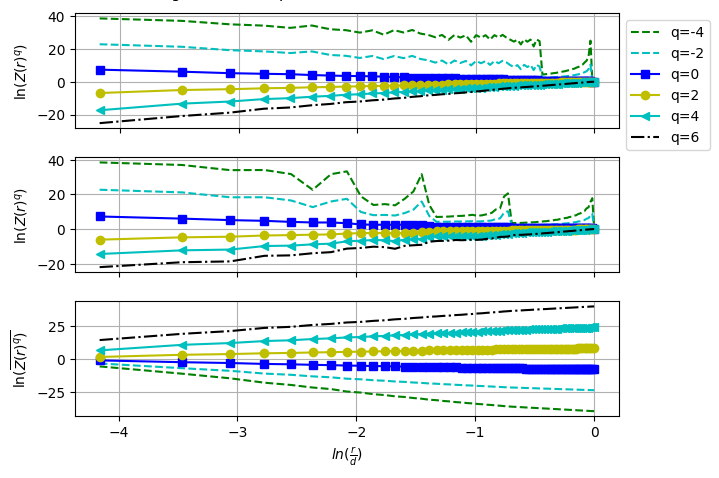
\includegraphics[scale=0.7]{Capitulo4Multifractalidad/imagenes/a_TqLnrBCflower22.png}
    \caption{Regresión lineal entre $\ln(Z_r(q)$ y $\ln(\frac{r}{b})$. De arriba hacia abajo, la primera figura corresponde al método BCFS, la segunda al método BCC y la tercera SB}
\end{figure}

\begin{figure}[H]
    \centering
    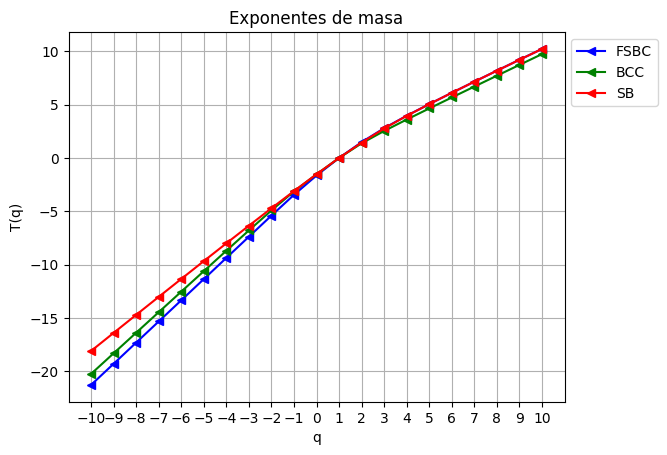
\includegraphics[scale=0.7]{Capitulo4Multifractalidad/imagenes/a_Tqflower22.png}
    \caption{Exponentes de masa para red real ecoli}
\end{figure}

\begin{figure}[H]
    \centering
    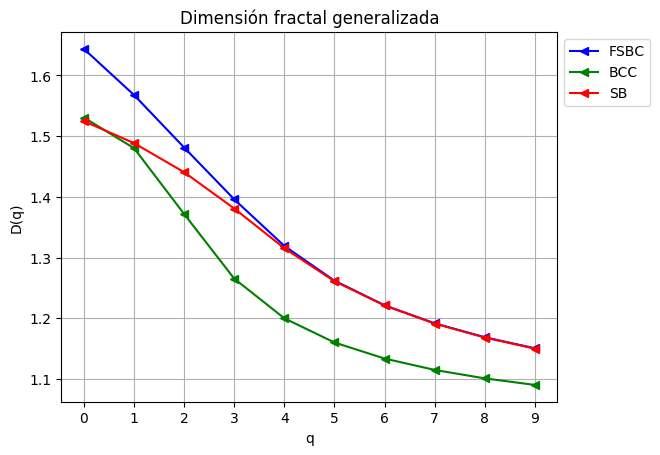
\includegraphics[scale=0.7]{Capitulo4Multifractalidad/imagenes/a_Dqflower22.png}
    \caption{Dimensión fractal generalizada para para red real ecoli}
\end{figure}

La dimensión fractal de esta red es 1.59


En el articulo sólo se realiza un análisis de gráficas, en el cual se indica que la red es levelmente multifractal. En en análisis del artículo se indica que la estructura en general es multifractal, ya que esta no es un fractal matemático, es decir que conserve su misma escala al infinito.

Los datos obtenidos de la red son.

\begin{table}[H]
    \centering
    \begin{tabular}{|c|c|c|c|}
        \hline
         \textbf{Dato}& \textbf{BCFS} & \textbf{BCC} & \textbf{SB} \\
         \hline
         Dimensión fractal & 1.64 & 1.53 & 1.52\\
         \hline
         Dimensión fractal generalizada  & 1.56 & 1.48 & 1.48\\
         \hline
         Dimensión de correlación & 1.48 & 1.37 & 1.44\\
         \hline
         Dimensión máxima & 1.92 & 1.83 & 1.64 \\
         \hline
         Dimensión mínima & 1.13 & 1.83& 1.13 \\
         \hline
         Variación en la dimensión & 0.79 & 0.74 & 0.51 \\
         \hline
    \end{tabular}
    \caption{Comparación de los datos obtenidos de los diferentes métodos de análisis multifractal}
\end{table}


\section{Estrategias evolutivas}
\label{cap4:evolutivo}

La idea de esta estrategia es buscar los centros de cajas directamente, de tal forma el algoritmo no deba realizar repeticiones

\subsection{El algoritmo}

El genotipo del algoritmo es un arreglo de enteros, el cual indica los nodos que van a ser centros de cajas. Este tiene tamaño entre el 40\% y 80\% del número total de nodos de la red.

\begin{equation}
    [a_1,a_2,a_3,\cdots,a_n]
\end{equation}

El fenotipo es los centros de las cajas sobre los cuales se va calcular el algoritmo.

\subsubsection{Población inicial}

La población inicial son $k$ individuos, cada uno de los cuales es una selección aleatoria de nodos sin repetir.

\subsubsection{Función de evaluación}

La evaluación de un individuo consiste en dos factores:

\begin{itemize}
    \item El grado de cada uno de los centros, entre mayor sea, mayor puntaje tiene el individuo
    \item La distancia entre los centros, se busca que estén lo más alejados posibles
\end{itemize}

Un individuo es calificado de acuerdo a la suma de estos factores

\subsubsection{Operadores}

Para el cruce, se hace una selección por ruleta\cite{9788497321839}, el cruce entre dos individuos se genera de la siguiente forma:

\begin{enumerate}
    \item Se toman los nodos de los dos padres y se incluyen en un conjunto
    \item Se toman nodos aleatorios de este conjunto para generar un hijo
\end{enumerate}

De esta forma, se cruzan los individuos para garantizar se tengan hijos válidos. En cada generación se crean ún numero determinado de nuevos individuos, el cual es especificado como entrada al algoritmo.

Para la mutación, se selecciona un nodo de un individuo y se cambia por otro, conservando que no sea igual a otro nodo.

\subsubsection{Cambio de población}

Se eliminan los individuos con peor valor de función de evaluación, los cuales son reemplazados por los nuevos individuos creados en el cruce.


\subsubsection{Criterio de parada}

Se manejan dos criterios de parada, los cuales son entradas al algoritmo:

\begin{itemize}
    \item Un número de iteraciones especificado por le usuario
    \item Un criterio que consiste en observar si en un número determinado de iteraciones, no se presenta mejora en el mejor individuo
\end{itemize}


\section{Estrategias Recocido Simulado}

Este algoritmo tiene la misma estrategia del algoritmo evolutivo, la diferencia radica en que iniciamos con un estado aleatorio y aceptamos el estado de acuerdo a la función de evaluación y a la temperatura del sistema.

El estado está descrito en términos de un conjunto de nodos de tamaño definido por el usuario, los cuales representan los centros de las cajas.

A diferencia del algoritmo evolutivo, en cada iteración comparamos el estado con un estado vecino. Este estado vecino se crea tomando aleatoriamente uno de los nodos del estado actual y cambiándolo por un nodo vecino en la red, conservando que los nodos no se repitan.
\section{Estudio de los algoritmos de inteligencia artificial}

\label{cap4:analisisIA}

Los algoritmos Genético y de Recocido simulado son comparados aplicando pruebas en las mismas redes seleccionadas de la sección \ref{sec:cap4analisis}

En el caso del algoritmo genético también es mostrada la evolución de la función de evaluación.


\subsection{Red libre de escala}

\begin{figure}[H]
    \centering
    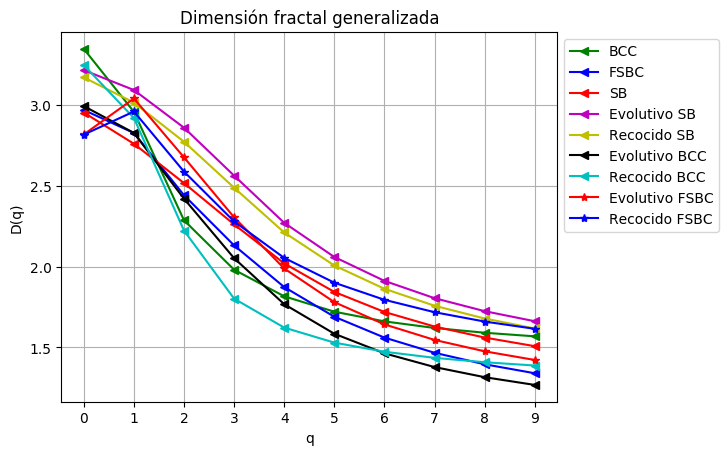
\includegraphics[scale=0.7]{{Capitulo4Multifractalidad/imagenesIA/grafica_Dq20180506_035455ScaleFree4000Nodes}.png}
    \caption{Multifractalidad en red libre de escala con 4000 nodos}
\end{figure}

\begin{figure}[H]
    \centering
    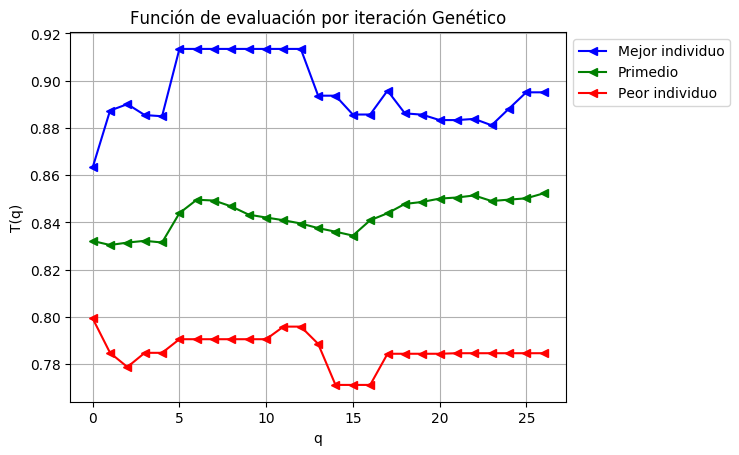
\includegraphics[scale=0.7]{{Capitulo4Multifractalidad/imagenesIA/grafica_Fitness20180502_203759ScaleFree2000Nodes.txt}.png}
    \caption{Evolución de la función de evaluación en red libre de escala con 4000 nodos}
\end{figure}

\subsection{Red de mundo pequeño}

\begin{figure}[H]
    \centering
    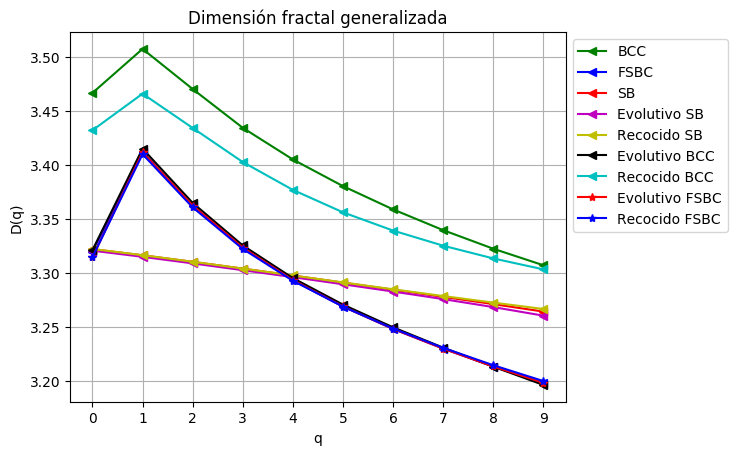
\includegraphics[scale=0.7]{{Capitulo4Multifractalidad/imagenesIA/grafica_Dq20180506_141058SmallWorld5000NodesRewire01.txt}.png}
    \caption{Multifractalidad en red de mundo pequeño de 5000 nodos con p = 10\%}
\end{figure}

\begin{figure}[H]
    \centering
    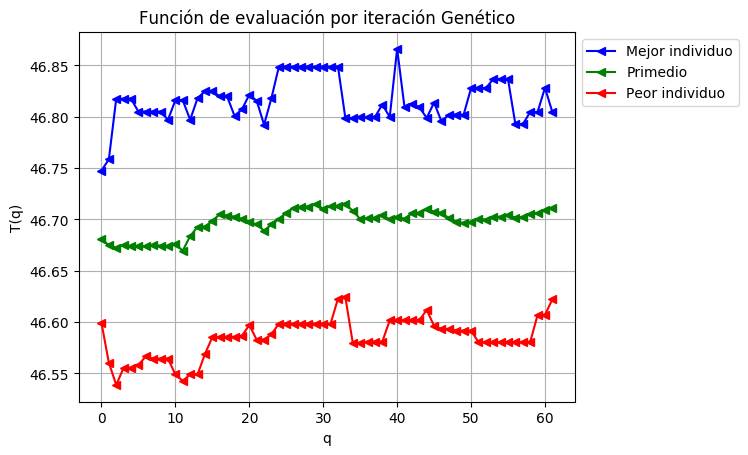
\includegraphics[scale=0.7]{{Capitulo4Multifractalidad/imagenesIA/grafica_Fitness20180506_141058SmallWorld5000NodesRewire01.txt}.png}
    \caption{Evolución de la función de evaluación en red de mundo pequeño de 5000 nodos con p = 10\%}
\end{figure}

\subsection{Red aleatoria}

\begin{figure}[H]
    \centering
    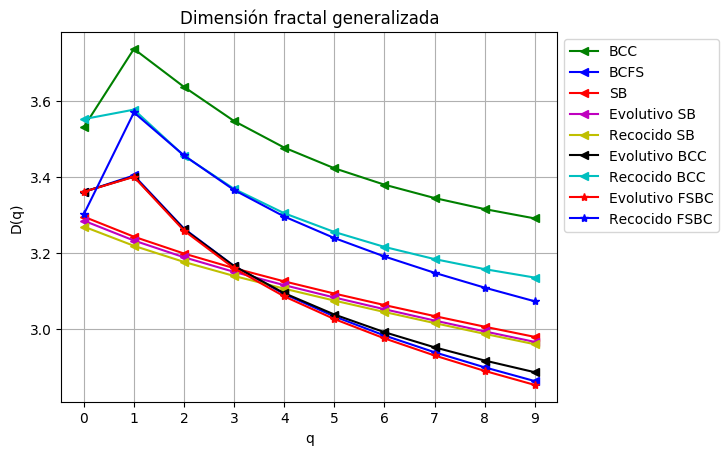
\includegraphics[scale=0.7]{{Capitulo4Multifractalidad/imagenesIA/grafica_Dq20180502_133953Random1991Nodes5939}.png}
    \caption{Multifractalidad en red aleatoria con 5620 nodos}
\end{figure}

\begin{figure}[H]
    \centering
    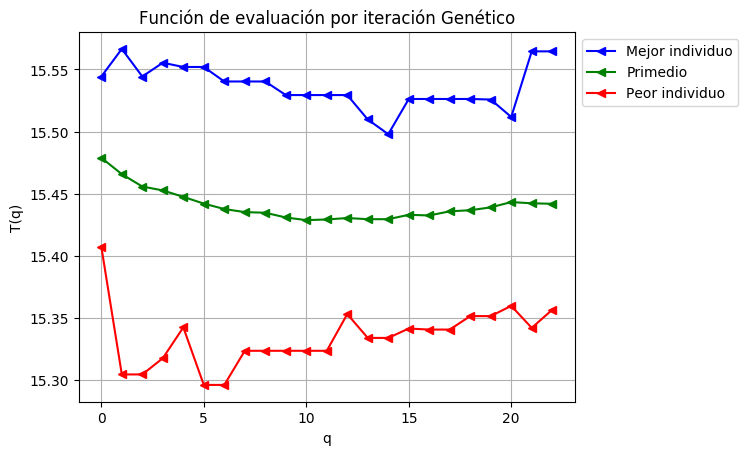
\includegraphics[scale=0.7]{{Capitulo4Multifractalidad/imagenesIA/grafica_Fitness20180508_231031Random3373Nodes5978.txt}.png}
    \caption{Evolución de la función de evaluación en red aleatoria con 5620 nodos}
\end{figure}

\subsection{Red observada bacteria Ecoli}

\begin{figure}[H]
    \centering
    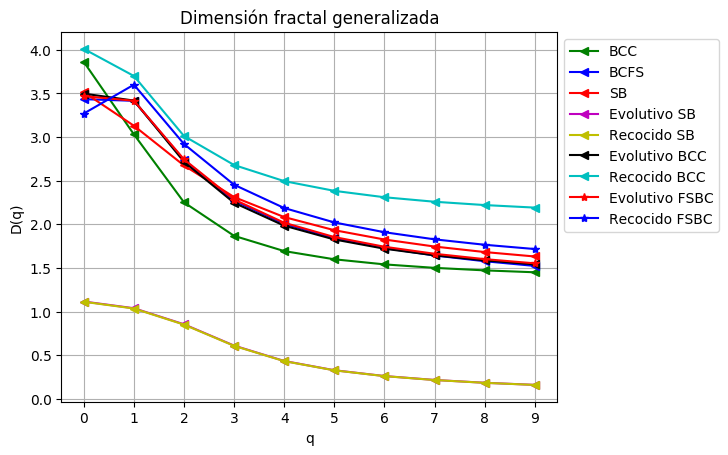
\includegraphics[scale=0.7]{{Capitulo4Multifractalidad/imagenesIA/grafica_Dq20180504_000006EColi}.png}
    \caption{Multifractalidad en red observada de Ecoli}
\end{figure}

\begin{figure}[H]
    \centering
    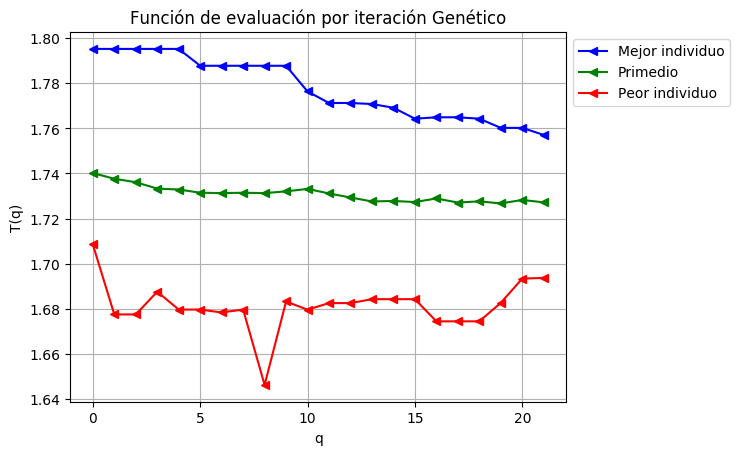
\includegraphics[scale=0.7]{{Capitulo4Multifractalidad/imagenesIA/grafica_Fitness20180508_182332cerevisiae.txt}.png}
    \caption{Evolución de la función de evaluación en red observada de Ecoli}
\end{figure}

\subsection{Red fractal}

\begin{figure}[H]
    \centering
    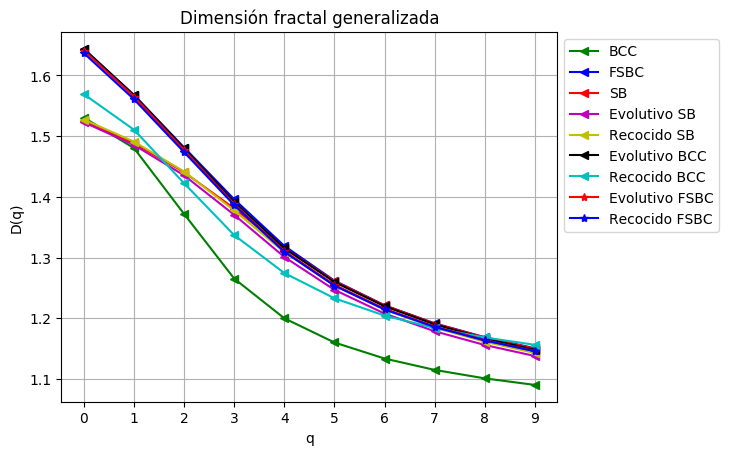
\includegraphics[scale=0.7]{{Capitulo4Multifractalidad/imagenesIA/grafica_Dq20180511_101739floweru2v2}.png}
    \caption{Multifractalidad en red generada fractal (2,2)-flower}
\end{figure}

\begin{figure}[H]
    \centering
    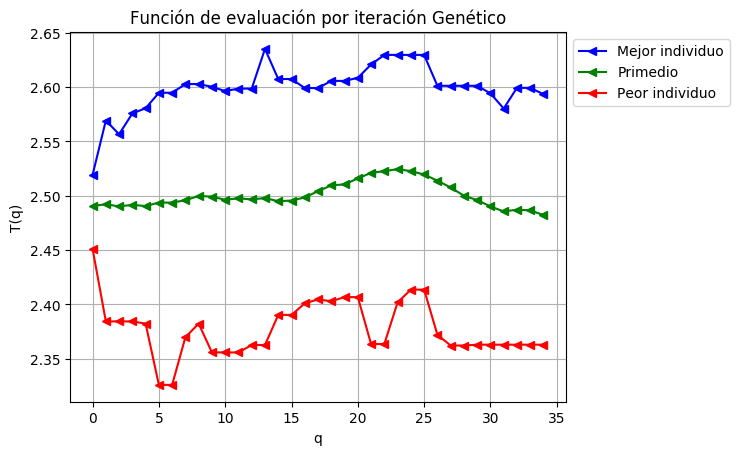
\includegraphics[scale=0.7]{{Capitulo4Multifractalidad/imagenesIA/grafica_Fitness20180511_101739floweru2v2.txt}.png}
    \caption{Evolución de la función de evaluación en red fractal (2,2)-flower}
\end{figure}

\subsection{Análisis de los algoritmos}

Se puede observar que:

\begin{enumerate}
    \item No es sencillo estimar un número de iteraciones para los algoritmos de inteligencia artificial, en algunos casos el resultados es muy cercano a los deterministas, en otros no.
    \item Dado que el tiempo requerido para la ejecución de los algoritmos es considerable (más de 100 horas) de acuerdo a tabla \ref{tab:executionTimes}, se requiere un soporte teórico para conocer el número de iteraciones óptimo para cada estrategia.
    \item Las gráficas de la evolución de la función de evaluación muestran que la heurística usada debe ser mejorada para validar cuales son los mejores centros. se observa una convergencia en las primeras generaciones.
\end{enumerate}

\section{Análisis de los tiempos de ejecución}

En la tabla \ref{tab:executionTimes} son analizados los tiempos de ejecución de cada uno de los algoritmos, de acuerdo al protocolo de pruebas especificado en el Anexo B de la página \pageref{AnexoB}

\begin{table}[H]
    \centering
    \begin{tabular}{|p{1cm}|p{1cm}|p{1.1cm}|p{1cm}|p{1.5cm}|p{1.5cm}|p{1.5cm}|p{1.5cm}|p{1.5cm}|p{1.5cm}|}
         \hline
         \textbf{Red} & \textbf{BCFS} & \textbf{BCC} & \textbf{SB} & \textbf{Genético BCFS} & \textbf{Recocido BCFS} &
         \textbf{Genético BCC} & \textbf{Recocido BCC} &
         \textbf{Genético SB} & \textbf{Recocido SB} \\
         \hline
         Red A & 10788 & 10715 & 1193 & 7097 & 5092 & 6324 & 4995 &4644 & 6653 \\
         \hline
         Red B & 84833 & 85043  & 16598  & 48511  & 38744  &  35022 & 48511 & 35067 & 48360  \\
         \hline
         Red C & 271062 & 380427 & 19535  &  16508 & 20410  &  27972 & 16508 & 24480 & 15692  \\
         \hline
         Red D & 106396 & 106751 &  60063 & 75580  & 61520  & 94662  & 57915  & 68997 &  60096 \\
         \hline
         Red E & 494803 & 394747 &  8430 & 13698  & 10614  & 31047  & 11136  & 14146 &  10448 \\
         \hline
    \end{tabular}
    \caption{Tiempos de ejecución para diferentes redes en segundos}
    \label{tab:executionTimes}
\end{table}

Se observa que en general los algoritmos BCFS y BCC tienen una mejora considerable cuando se les aplica estrategias de inteligencia artificial. Con respecto al algoritmo SB, se requiere realizar un estudio más amplio para llegar a una conclusión debido a que:

\begin{itemize}
    \item El número de iteraciones de SB depende del número de nodos y del número de repeticiones del algoritmo.
    \item El número de iteraciones de los algoritmos de IA depende los parámetros suministrados por el usuario.
\end{itemize}

Lamentablemente, los algoritmos requiere gran capacidad de cómputo y tiempo de ejecución, por lo que esto se debe realizar en un estudio posterior.
\newpage
\section{Resumen y conclusiones del capítulo}

En este capitulo, inicialmente se analizan 3 algoritmos presentes en la literatura: Fixed Size Box Counting (FSBC), Box Compact Counting (BCC) y SandBox (SB), estos métodos no son precisos para determinar la dimensión fractal, ya que dentro de sus pasos hay una selección aleatoria de centros de cajas. Por lo tanto, debe repetirse un gran número de veces para obtener un mejor resultado.

La herramienta provista por estos algoritmos, permite caracterizar si una red es multifractal o monofractal en su estructura, se encuentra que:

\begin{itemize}
    \item Redes libres de escala, son multifractales, algo que es esperado debido a que se pueden describir a través de componentes centrados en los hubs
    \item Redes de mundo pequeño, son monofractales, ya que son compactas debido a que su construcción busca reducir el diámetro de los caminos entre los nodos
    \item Las redes aleatorias, no se puede caracterizar con estas medidas
\end{itemize}

Ninguno de los algoritmos estudiados garantiza un valor preciso de la dimensión fractal debido a que requieren realizar una búsqueda intensiva dentro de las redes y esto es impráctico en redes grandes.

Estos algoritmos requieren un gran tiempo de cómputo, el cual depende del número de nodos y aristas, por lo que proveer una medida de complejidad es muy impreciso. En consecuencia, se comparan estos algoritmos utilizando el tiempo de cómputo en distintos ejemplos.

Como estrategia para reducir el tiempo de cómputo, se propone un algoritmo evolutivo y uno de recocido simulado, la idea es mediante un proceso distinto al de cubrimiento de cajas que debe estudiar toda la red elegir los centros de las cajas. La estrategia se basa en una heurística que consiste en buscar una configuración de nodos, los cuales tengan el mayor grado posible y se encuentren lo más alejados entre sí que sea posible.

Los resultados de la tabla \ref{tab:executionTimes}, indican que las estrategias de inteligencia artificial mejoran el tiempo de ejecución de los algoritmos FSBC y BCC: Para el algoritmo SB, debido a que depende de una selección aleatoria, no se puede concluir si las estrategias lo mejoran o no.

%%%%%Capitulo Cinco: Medición de Robustez%%%%%%%%
\chapter{Medición de la robustez}\label{cap5}

\markboth{Medición de la robustez}{Medición de la robustez}

\section{Análisis de robustez}

\subsubsection{Medidas de robustez}


Medidas que hay 

Mismas gráficas de Hernán

Solo robustez

\subsubsection{Estrategias de simulación de ataques}


Para las mismas redes
\section{Ataque evolutivo}
\section{Estrategias simulated Annealing}

%%%%%%Capitulo Seis: Multifractalidad y robustezo%%%%%%%%%%%%%%%%%%%%%
\chapter{Multifractalidad y robustez}\label{cap6}
\markboth{Multifractalidad y robustez}{Multifractalidad y robustez}


\section{Análisis multifractal}

\subsection{Comparativa entre algoritmos SandBox y BoxCounting}

\subsection{Comparativa entre estrategias de inteligencia artificial y SandBox}

\subsection{Comparativa entre estrategias de inteligencia artificial y Boxcouting}

\subsection{Discusión de resultados}

\section{Análisis de robustez}

\subsection{Comparativa estrategias de ataque de la literatura y de inteligencia inteligencia artificial}

\subsection{Relación multifractalidad y robustez}

\subsection{Discusión de resultados}


%%%%%Capitulo Siete: Implementacion%%%%%%%%
\chapter{Implementación de la librería} \label{cap7}
\markboth{Implementación de la librería}{Implementación de la librería}

\section{Desarrollo de la librería}

\subsection{Procesamiento de redes con SNAP}

\subsubsection{¿Porque SNAP?}
%https://www.researchgate.net/post/Which_open_source_software_is_best_for_network_data_analysis


\subsubsection{Funciones utilizadas}

\subsection{Desarrollo de las funciones}



\subsection{Arquitectura de la librería}
\section{Requerimientos de la librería}


\subsection{Dependencias de software}

\subsection{Recomendaciones de capacidad de cómputo}
\section{Funciones provistas}

\subsection{Análisis multifractal}

\subsection{Análisis de robustez}

\subsection{Algoritmos evolutivos}

\subsection{Algoritmos de inteligencia artficial}
\section{API}

\subsection{Desarrollo del API}


\subsection{Recomendaciones de uso}





%%%%CAPITULO A: Conclusiones y trabajos futuros

\chapter{Conclusiones y trabajos futuros}\label{cap9}
\markboth{Conclusiones y trabajos futuros}{Conclusiones y trabajos futuros}

\section{Conclusiones}

\begin{enumerate}
    \item Las redes de mundo pequeño muestran una estructura monofractal y conservan su estructura a media que son atacadas, esto debido a que son compactas. Esto es un resultado interesante, ya que además de la medida de distancia promedio de las distancias más cortas entre los nodos, se puede utilizar el análisis de multifractal y de robustez para caracterizar estas redes. En las pruebas realizadas, evidencia que en las estrategias de ataque por centralidad, se muestra un efecto en la estructura de la red.
    \item Las relación entre multifractalidad y robustez está dada, que a medida una red pierde nodos, la dimensión fractal de las estructuras presentes en la red va tendiendo a 0 y a una característica monofractal. Esto indica una descomposición de las estructuras de la red; siendo el caso más relevante el de las redes libres de escala a medida que pierden los nodos con mayor grado.
    \item Las diferentes estrategias de análisis multifractal muestran variaciones en el cálculo de las dimensiones fractales, esto se debe a que los centros se establecen aleatoriamente, lo que puede producir diferentes resultado de acuerdo a la red. Sin embargo, permite caracterizar las redes de acuerdo a su estructura, ya que entre más pronunciada sea la curva de la dimensión fractal, más diferencias estructurales existen dentro de la red.
    \item En general, las estrategias de inteligencia artificial permiten estimar centros de cajas de las redes, lo que permite mejorar el tiempo de cómputo de los algoritmos BCC y BCFS, sin embargo, tienen problemas de precisión, ya que encontrar los centros es un proceso iterativo que depende del número de nodos y la forma en que se interconectan. Al aumentar el número de iteraciones de los algoritmos se mejora la precisión, sin embargo, el costo computacional debe ser considerado, ya que los cálculos podrían tomar una gran cantidad de tiempo.
    \item Las estrategias de inteligencia artificial demostraron mejores tiempos de ejecución de los algoritmos BCC y BCFS en el caso del análisis multifractal. Sin embargo, para el caso de SB los resultados no son concluyentes, debido a que las redes estudiadas no son los suficientemente grandes para llegar a un resultado concreto.
    \item Para el análisis de la robustez, los algoritmos de IA no mostraron ser una estrategia de ataque que produzca más efectos en la estructura de la red que las basadas en el grado y la centralidad de los nodos. Esto se debe a que en las redes estudiadas los nodos que tienen mayor valor de centralidad, son claves para la transmisión de información dentro de la red.
    \item El uso de librerías con representaciones comprimidas de las redes, provee un marco de trabajo para el desarrollo de algoritmos para el análisis de multifractalidad, ya que al reducirse la complejidad espacial y computacional se realizan las búsquedas dentro de las redes con mayor rapidez que con otras opciones disponibles.
\end{enumerate}
\newpage
\section{Trabajos futuros}

\begin{itemize}
    \item Debe establecerse un método analítico para validar el análisis multifractal de los diferentes métodos, como se vio en las diferentes pruebas los resultados pueden variar significativamente
    \item El algoritmo de SandBox propuesto por Liu\cite{Liu2015}, es el que mejor resultados presenta en las pruebas realizadas, sin embargo, no se puede asegurar tenga mejor rendimiento que las técnicas de Inteligencia Artificial propuestas, por lo que se requiere un estudio a profundidad de este tema.
    \item Se debe proponer una estrategia para generar una heurística que permita seleccionar los centros de las cajas, ya que la propuesta de este trabajo depende si la red tiene estructura libre de escala, ya que se buscan nodos altamente conectados.
    \item A partir del trabajo realizado, una idea interesante a explorar son los generadores de redes monofractales y robustas, los cuales deben conservar su estructura ante diferentes estrategias de ataque. Esto permite generar un marco de trabajo para el diseño de redes con alta tolerancia a fallos.
    \item En el caso de las redes libres de escala debe realizarse un estudio variando el término de la ley de potencia.
    \item Las pruebas de este trabajo deben ejecutarse en un entorno con mayor capacidad de cómputo, ya que los resultados encontrados en algunos casos no corresponden a lo esperado, ya que los algoritmos requieren iterar una gran cantidad de veces para obtener resultados cercanos a los algoritmos presentes en la literatura.
    \item Se deben proponer estrategias de distribución de los cálculos, ya que el análisis multifractal depende de la configuración de cajas a un radio dado $r$, este valor puede ser distribuido, ya que no hay dependencias entre ellos. Así mismo, para la robustez se puede probar con diferentes porcentajes de perdidas de nodos y realizar el respecto análisis multifractal.
\end{itemize}


%%%%%BIBLIOGRAFIA%%%%%%%%
\bibliography{Bibliografia}


%%%%%%%%%%%%%%%%%%%%%%%%%%%%%%%%%%%%%%%%%%%%%ANEXOS%%%%%%%%%%%%%%%%%%%%%%%%%%%%%%%
\chapter*{Anexos}
\addcontentsline{toc}{chapter}{Anexos}
\markboth{Anexos}{Anexos}

\section*{Anexo A: Descripción de redes de prueba}
\addcontentsline{toc}{section}{Anexo A: Descripción de redes de prueba}
\label{AnexoA}

Para este trabajo se han utilizado las redes de prueba del articulo de Wang\cite{Wang2014}. Estas son descritas a continuación en la tabla \ref{tab:redesPrueba}.



\begin{longtable}{|p{2cm}|p{2cm}|p{2cm}|p{2cm}|p{2cm}|p{4cm}|}
\hline
    \textbf{Tipo} & \textbf{Número de vértices} & \textbf{Número de aristas} & \textbf{Diámetro} & \textbf{Diámetro camino promedio más corto} & \textbf{Descripción}\\
    \hline
     \endhead
    Libre de escala & 2000 & 1999 & 19 & 10.14 & Generada con modelo Barabasi-Albert. Parámetro de ley de potencia 1.94. \\
    \hline
    Libre de escala & 4000 & 3999 & 22 & 11.91 & Generada con modelo Barabasi-Albert. Parámetro de ley de potencia 2.04. \\
    \hline
    Libre de escala & 8000 & 7999 & 23 & 10.95 & Generada con modelo Barabasi-Albert. Parámetro de ley de potencia 1.98. \\
    \hline
    Mundo pequeño & 5000 & 24997 & 11 & 7.87 & Generada con modelo Watts-Strogatz, con probabilidad de reconexión del 5\% \\
    \hline
    Mundo pequeño & 5000 & 25000 & 9 & 6.4 & Generada con modelo Watts-Strogatz, con probabilidad de reconexión del 10\% \\
    \hline
    Mundo pequeño & 5000 & 24996 & 7 & 5.43 & Generada con modelo Watts-Strogatz, con probabilidad de reconexión del 20\% \\
    \hline
    Aleatoria & 1991 & 5939 & 8 & 4.95 & Generada con modelo Erdos-Renyi \\
    \hline   
    Aleatoria & 3373 & 5978 & 8& 7.69 & Generada con modelo Erdos-Renyi \\
    \hline
    Aleatoria & 5620 & 8804 & 14 & 8.84 & Generada con modelo Erdos-Renyi \\
    \hline  
    Biológica observada & 3954 & 7810 & 12 & 5.07 & Red de iteraciones de proteínas de la bacteria intestinal C.elegans obtenida desde Biogrid\cite{biogrid}\\
    \hline  
    Biológica observada & 5176 & 22624 & 9 & 4.75 &  Red de de iteraciones de proteínas del hongo cerevisiae obtenida desde DIP \cite{dipcite}\\
    \hline  
    Biológica observada & 2940 & 11627 & 10 & 4.93 & Red de las iteraciones de proteínas de Ecoli obtenida desde DIP\cite{dipcite}\\
    \hline  
    Fractal & 2732 & 4096  & 64 & 57.15 & Séptima generación de (2,2)-flower\\
    \hline  
    Fractal & 2732 & 4096 & 12 & 7.87 & Séptima generación de (1,3)-flower\\
    \hline  
\caption{Redes utilizadas en el proyecto}
\label{tab:redesPrueba}
\end{longtable}

Las redes reales fueron procesadas con el software Cytoscape\cite{cytoscope} para generar la red asociada no dirigida y posteriormente con Gephi\cite{gephi} para transformarlas en formato PAJEK.

\newpage
\section*{Anexo B: Descripción de protocolos de prueba}
\addcontentsline{toc}{section}{Anexo B: Descripción de protocolos de prueba} 
\label{AnexoB}
\section*{Anexo C: Pruebas}
\addcontentsline{toc}{section}{Anexo C: Pruebas} \label{AnexoC}

\subsection*{Multifractalidad}
\addcontentsline{toc}{subsection}{Multifractalidad}


\end{document}
